\documentclass[a4paper,11pt]{article}
\usepackage[T1]{fontenc}
\usepackage[utf8]{inputenc}
\usepackage{newtxtext,newtxmath}
\usepackage{amsfonts, mathrsfs, microtype}
\usepackage{amsmath, bm}
\usepackage[showonlyrefs]{mathtools}
\usepackage{paralist, parskip}
\usepackage{todonotes}
\usepackage{graphicx, subfig, rotating, booktabs, multirow, url}
\usepackage[no-weekday]{eukdate}
\usepackage[linesnumbered,lined,boxed,commentsnumbered]{algorithm2e}
\usepackage{tikz}
\usepackage{comment}
\usepackage{natbib}
\usepackage{titling}
\usepackage{blindtext}
\usepackage{chemformula}
\usepackage{textcomp}
%\usepackage[section]{placeins}

\SetKwInOut{Parameter}{parameter}
\setlength{\algomargin}{2em}

\newif\ifxyz
\def\xyztrue{\let\ifxyz\iftrue}
\def\xyzfalse{\let\ifxyz\iffalse}
%\let\ifxyz\iftrue
\let\ifxyz\iffalse

\usepackage[margin=3cm]{geometry}

\usetikzlibrary{shapes.geometric, arrows}
\tikzstyle{standard} = [rectangle, rounded corners, minimum width=1.5cm, minimum height=2cm,text width=2.5 cm, text centered, draw=black, fill=black!5]

\tikzstyle{state} = [ellipse, rounded corners, minimum width=1.5cm, minimum height=2cm,text width=1.5 cm, text centered, draw=black, fill=black!5]
\tikzstyle{io} = [trapezium, trapezium left angle=70, trapezium right angle=110, minimum width=3cm, minimum height=1cm, text centered, draw=black, fill=blue!30]
\tikzstyle{process} = [rectangle, minimum width=3cm, minimum height=1cm, text centered, text width=3cm, draw=black, fill=orange!30]
\tikzstyle{decision} = [diamond, minimum width=3cm, minimum height=1cm, text centered, draw=black, fill=green!30]
\tikzstyle{arrow} = [thick,->,>=stealth]
\tikzstyle{bigbox} = [rectangle, rounded corners, minimum width=1.5cm, minimum height=6cm,text width=3 cm, text centered, draw=black, fill=black!5]

%% CAPTIONS
\RequirePackage{caption}
\DeclareCaptionStyle{italic}[justification=centering]
 {labelfont={bf},textfont={it},labelsep=colon}
\captionsetup[figure]{style=italic,format=hang,singlelinecheck=true}
\captionsetup[table]{style=italic,format=hang,singlelinecheck=true}

%% LINE AND PAGE BREAKING
\allowdisplaybreaks
\sloppy
\clubpenalty = 10000
\widowpenalty = 10000
\brokenpenalty = 10000

%% GRAPHICS
\RequirePackage{graphicx}
\setcounter{topnumber}{2}
\setcounter{bottomnumber}{2}
\setcounter{totalnumber}{4}
\renewcommand{\topfraction}{0.85}
\renewcommand{\bottomfraction}{0.85}
\renewcommand{\textfraction}{0.15}
\renewcommand{\floatpagefraction}{0.7}
%\RequirePackage[section]{placeins}

\DeclareMathOperator*{\argmin}{arg\,min}
\DeclareMathOperator*{\argmax}{arg\,max}
\DeclareMathOperator*{\E}{E}

% =======================================================================
\begin{document}
% =======================================================================
\title{\bf{Early classification of spatio-temporal events \\ using partial information}}
\author{Sevvandi Kandanaarachchi$^1$ \\ Rob J Hyndman$^1$ \\ and \\ Kate Smith-Miles$^2$}
\date{%
	\scriptsize{ $^1$Department of Econometrics and Business Statistics, Monash University, Clayton VIC 3800, Australia.\\%
		$^2$School of Mathematics and Statistics, The University of Melbourne, Parkville, VIC 3010, Australia\\[2ex]}%
	\today
}

\begin{titlingpage}
	\maketitle
	\begin{abstract}
		This paper investigates event extraction and early event classification in contiguous spatio-temporal data streams, where events need to be classified using partial information, i.e.\ while the event is ongoing. The framework incorporates an event extraction algorithm and an early event classification algorithm. We apply this framework to synthetic and real problems and demonstrate its reliability and broad applicability. The algorithms and data are available in the R package \textit{eventstream}, and other code in the supplementary material.
	\end{abstract}
\end{titlingpage}

\newgeometry{top=2cm,bottom=2cm,right=2cm,left=2cm}

% =======================================================================
\section{Introduction}
% =======================================================================

Early detection and classification of emerging events in data streams is an important challenge in our data-rich world. Data streams may arise from many different applications including social media, Internet of Things, video surveillance, epidemiology and wireless sensors, to name a few. In each of these diverse applications, there are typically events that occur and are of interest because of their disruptive behaviour to the system.

In particular, we are interested in events that start, develop for some time, and stop at a certain time. Such events can be characterised by measurable properties or features, including the ``age'' of the event. It is a challenge to classify these events while they are still developing because only partial information is available at this stage. Once the events have stopped developing --- when the events are finished --- it is easier to classify them as the complete event features are now available. For example, it is easier to differentiate a daffodil from a tulip when both are in full bloom, but more difficult to differentiate a daffodil bud from a tulip bud without resorting to other information such as characteristics of leaves. Another example is identifying a network intrusion attack in its early stages. While it may be easier to identify a breach after it has happened, it is more difficult to identify which bits of network traffic is causing the breach while it is happening \citep{suthaharan2014big}.

\begin{figure}[!ht]
	\centering
	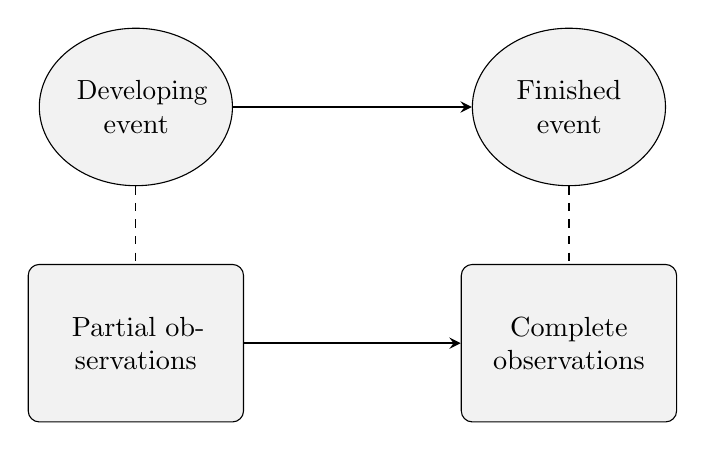
\begin{tikzpicture}[node distance=2cm, auto]
		\node (dev) [state] {Developing event};
		\node (fin) [state, right of=dev, xshift=3.5cm] {Finished event};
		\draw [arrow] (dev) -- (fin);
		\node (pobs) [standard, below of=dev, yshift=-1cm]{Partial observations};
		\node (fullobs) [standard, right of=pobs, xshift=3.5cm]{Complete observations};
		\draw [arrow] (pobs) -- (fullobs);
		\draw [dashed] (dev) -- (pobs);
		\draw [dashed] (fin) -- (fullobs);
	\end{tikzpicture}
	\caption{Event states and partial observations.}
  \label{fig:0_1}
\end{figure}

In this regard, we can think of these events as having two states: developing and finished (Figure~\ref{fig:0_1}). The partial information contained in the developing events give rise to partial or premature observations, while the finished events give rise to complete observations. As the event develops, it gives rise to a series of partial observations --- each partial observation encapsulating more information than its predecessor --- culminating with the complete observation (Figure~\ref{fig:0_2}). Thus partial observations vary with the age of the event, the difference between the current time and the start time of the event. If early classification is important, one needs to take partial observations into account in the classification process. While event detection in data streams has received much attention from different disciplines ranging from video surveillance to social media \citep{medioni2001event, li2012tedas}, there has been little exploration on developing/premature event classification to the best of our knowledge.

\begin{figure}[!ht]
	\centering
	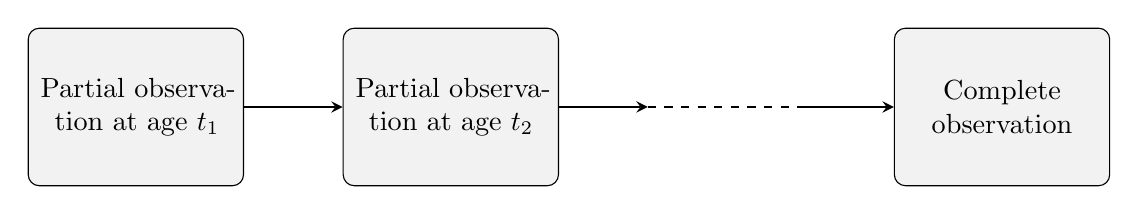
\begin{tikzpicture}[node distance=2cm, auto]
		\node (pobst1) [standard]{Partial observation at age $t_1$};
		\node (pobst2) [standard, right of=pobst1, xshift=2cm]{Partial observation at age $t_2$};
		\node (fullobs) [standard, right of=pobst2, xshift=5cm]{Complete observation};
		\draw [arrow] (pobst1) -- (pobst2);
		\draw [arrow] (pobst2) -- (6.5,0);
		\draw [arrow] (8.5,0) -- (fullobs);
		\draw[dashed] (6.5,0) -- (8.5,0);
	\end{tikzpicture}
	\caption{Partial observations growing with event-age.}
  \label{fig:0_2}
\end{figure}

A general framework for event classification in data streams comprises different stages:
\begin{inparaenum}
	\item data pre-processing;
	\item event detection and extraction;
	\item feature computation; and
	\item event classification.
\end{inparaenum}
This framework, augmented with partial observations, gives the additional functionality of early event classification as depicted in Figure~\ref{fig:1_1}. In our framework we do not explicitly consider data pre-processing as a separate stage as this is highly dependent on the application.

\begin{figure}[!htb]
	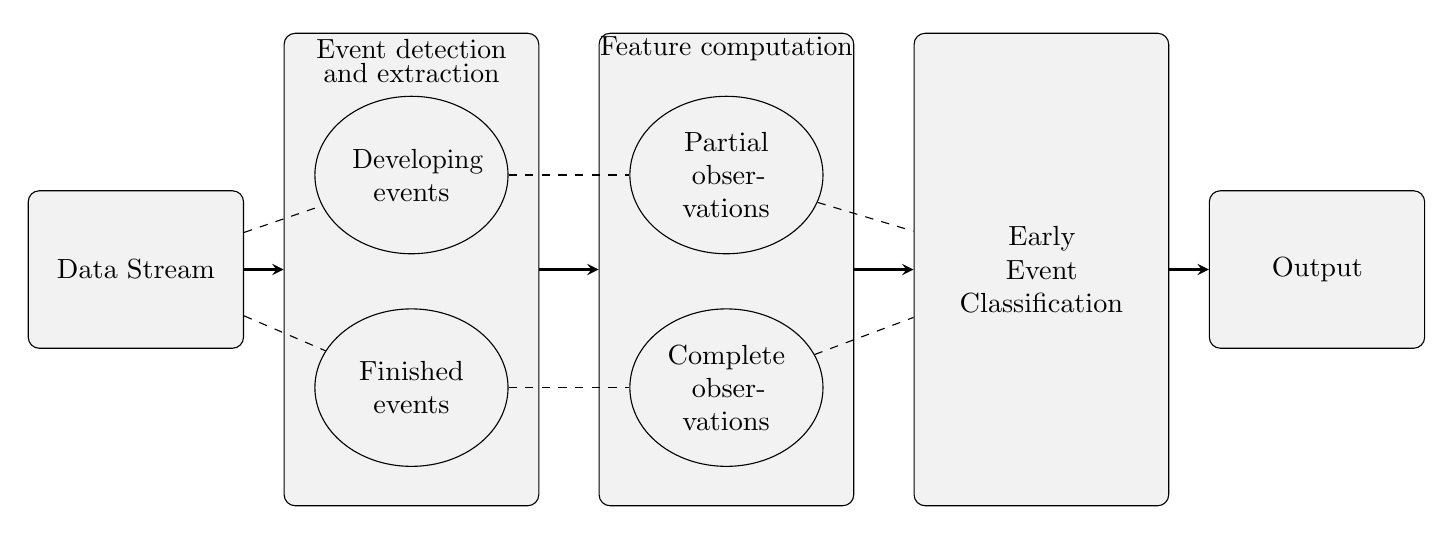
\begin{tikzpicture}[node distance=2cm]
		\node (start) [standard] {Data Stream};
		\node (extract) [bigbox, right of=start, xshift=1.5cm] {};
		\node (dummy)[above of=extract, yshift=0.8cm] {Event detection};
		\node (dummy)[above of=extract, yshift=0.5cm] {and extraction};
		\node (devEv) [state, right of=start, xshift=1.5cm, yshift=1.2cm]{Developing events};
		\node (finEv) [state, right of=start, xshift=1.5cm, yshift=-1.5cm]{Finished events};
		\node (features) [bigbox, right of=extract, xshift=2cm] {};
		\node (dummy)[above of=features, yshift=0.8cm] {Feature computation};
		\node (Pobs) [state, right of=devEv, xshift=2cm]{Partial observations};
		\node (Cobs) [state, right of=finEv, xshift=2cm]{Complete observations};
		\node (classify) [bigbox, right of=features, xshift=2cm] {Early \\ Event \\ Classification};
		\node (output) [standard, right of=classify, xshift=1.5cm] {Output};
		\draw [arrow] (start) -- (extract);
		\draw [arrow] (extract) -- (features);
		\draw [arrow] (features) -- (classify);
		\draw [arrow] (classify) -- (output);
		\draw[dashed] (devEv) -- (Pobs);
		\draw[dashed] (finEv) -- (Cobs);
		\draw[dashed] (Pobs) -- (classify);
		\draw[dashed] (Cobs) -- (classify);
		\draw[dashed] (start) -- (devEv);
		\draw[dashed] (start) -- (finEv);
	\end{tikzpicture}
	\caption{Framework for event extraction and classification for spatio-temporal data.}
  \label{fig:1_1}
\end{figure}

Fundamentally, early event classification can be tackled by embedding age-varying coefficients in a learned model \citep{hastie1993varying}. A linear model with age-varying coefficients is given by
\begin{equation}\label{eq:Int1}
	y_t = a_0(t) + a_1(t) x_1(t) + \cdots + a_b(t)x_b(t) + \varepsilon_t ,
\end{equation}
where $y_t$ is the output at age $t$, $a_i(t)$ are the age-varying coefficients, and $x_i(t)$ are the attributes of the event at age $t$; i.e.\ the partial/premature observation. A logistic model with age-varying coefficients is given by Equations~\eqref{eq:Int1} and~\eqref{eq:Int2}:
\begin{equation}\label{eq:Int2}
	z_t = e^{y_t}/(1 + e^{y_t})  ,
\end{equation}
where $z_t$ is the probability of the event being of a given class. As an event develops, the features $x_i(t)$ change with the age of the event, while keeping the class label constant. Thus, it is clear that the coefficients $a_i(t)$ need to change with the age of the event.

At this point, we note that concept drift \citep{gama2014survey} or non-stationarity of data streams \citep{hulten2001mining} is different from age-varying events. For non-stationary data streams the distribution of data changes with time. For example consider a fixed part of a river, which is monitored for fluctuations in water volume and for animals. In months of heavy rains, the water volume increases changing the distribution compared to previous months. This is an example of non-stationarity. In contrast, age-varying events are about the extracted events and not the data-stream. To continue with the same example, consider a log appearing on this portion of the river. When the log comes closer and the image becomes clearer, suppose it becomes apparent that it is not a log, but a crocodile. This is an example of an age-varying event. Clearly, from the time when the log appeared to the time when it was detected that it was a crocodile, no significant changes in water volume or the animal distributions took place. The volume of water and the average number of crocodiles in the river does not need to change when the perception of the log changed to that of a crocodile as a result of more information. Thus age-varying events comprise change within the event as a result of maturing partial observations, while non-stationarity concerns change within the data stream.

\subsection{Fibre optic cable example}\label{subsec:RealWorld}

We turn to an application where age-varying events occur. Figure~\ref{fig:Real_1} shows the heatmap of a dataset produced from a fibre optic cable. A pulse is periodically sent through the cable and this results in a data matrix where each horizontal row gives the strength of the signal at a fixed location $x_0$, and each vertical column gives the strength of the signal along the cable at a fixed time $t_0$. In this dataset the yellow parts represent high intensity values and the blue parts represent low intensity values.

\begin{figure}
	%	\centering
	\subfloat[][]{
		\includegraphics[width=0.49\textwidth]{./Graphics/Real_World.pdf}
    \label{fig:Real_1}
	}
	\subfloat[][]{
		\includegraphics[width=0.49\textwidth]{./Graphics/Two_Event_Features.pdf}
    \label{fig:Real_Feat_1} % width=0.49\textwidth, height=0.2\textheight width=0.48\linewidth
	}

	\caption{Figure~\ref{fig:Real_1} shows data from a fibre optic cable. We extract events from this dataset and compute event features. We consider two events belonging to two different classes and an event feature that changes with event-age. Figure~\ref{fig:Real_Feat_1} shows this event feature, which is the length to width ratio of the event, and how it changes with event-age.}
  \label{fig:Real_World_Data}
\end{figure}

Fibre optic sensor cables are used in many applications including optical communications, detecting undersea cable faults \citep{jiang2009technological}, detecting oil leakages \citep{nikles2004leakage}, detecting intruders on secured premises \citep{griffiths1995developments}, and monitoring health of infra-structure such as bridges and pipe-lines \citep{li2004recent}. Events in these applications can often be grouped into two classes. For example, a cable lying on the sea bed can produce spatio-temporal events that are either cable faults (A), or non-fault events due to the activity in the ocean (B)\@. Due to its sensitivity, fibre optic cables are also prone to noise. In a setting where early classification is important, we need to classify these events quickly, preferably while they are still ongoing.

In the dataset in Figure~\ref{fig:Real_1}, events are seen in the lighter-coloured parts. The event at approximately location 30 between the time interval 45 to 60 is of class A while other events that appear between locations 150 and 400 are of class B\@. Figure~\ref{fig:Real_Feat_1} shows an event feature, which is the length to width ratio of the event, computed on two events belonging to each class. As the event matures, we see this feature change with event-age and also that no single threshold can differentiate between the two events for all event ages. Due to the commercially sensitive nature of the dataset, we refrain from giving details about the actual application.

\subsection{Contributions}

We propose the framework depicted in Figure~\ref{fig:1_1}, which is summarized in Algorithm~\ref{algo:framework}, for early event detection, extraction and classification in contiguous spatio-temporal data streams using the partial observation structure.

Specifically, our contributions in this paper are:
\begin{enumerate}
	\item We introduce an algorithm for event detection and extraction  from contiguous spatio-temporal data. We use change point analysis and density based clustering to detect events. We call this algorithm Change-Point Density-Based Event Extraction (CPDBEE).
	\item We introduce a partial observations classifier suitable for early event classification. This classifier comprises multiple base classifiers, which are connected together using $L_2$ penalty terms. We refer to this Connected Classifier as CC\@.
	\item We demonstrate the validity of these algorithms on synthetic and real data and make the algorithms and data available in the R package \textit{eventstream} \citep{eventstream}
\end{enumerate}

\DontPrintSemicolon
\begin{algorithm}\fontsize{9}{10}\selectfont
	\SetKwInOut{Input}{input~~~}
	\SetKwInOut{Output}{output}
	\Input{~a 2 or 3-dimensional array denoting contiguous spatio-temporal data.}
	\Output{~events, event features and early classification results}
	Detect and extract developing and complete events from the data stream using CPDBEE (Sections~\ref{sec:EventExtract} and~\ref{sec:ResultsExtraction}). \\
	Compute event features. These are either partial or complete features computed from the extracted events (Section~\ref{sec:Featurelist}). \\
	Use the Connected Classifier CC for early classification of events (Sections~\ref{sec:ExtendedClassifier}--\ref{sec:Experiments}). \\
	\caption{\textit{Early event extraction and classification framework.}}
  \label{algo:framework}
\end{algorithm}

The remainder of the paper is organised as follows. Section~\ref{sec:RelatedWork} discusses related work in event detection, extraction and classification. In Section~\ref{sec:data} we introduce the datasets: synthetic data, fibre optic cable data, of which a portion is shown in Figure~\ref{fig:Real_World_Data}, and \ch{NO2} data from NASA's NEO \citep{OMINO2} website. We use all these datasets to demonstrate the effectiveness of the proposed event extraction and classification algorithms in subsequent Sections. We introduce our event detection and extraction algorithm CPDBEE in Section~\ref{sec:EventExtract} and discuss event extraction results in Section~\ref{sec:ResultsExtraction}. Section~\ref{sec:fts} presents the early classification framework by starting with event features in Section~\ref{sec:Featurelist}, followed by an explanation of partial observations in Section~\ref{sec:Notation}, and culminating with the connected classifier CC in Section~\ref{sec:ExtendedClassifier}. We discuss the early classification results in Section~\ref{sec:Experiments} and present our conclusions and discuss future work in Section~\ref{sec:Conclusions}. Section~\ref{sec:supmat} gives details on supplementary materials, which can be used to reproduce the results and Appendix~\ref{sec:App1} gives additional graphs of CPDBEE results.

% =======================================================================
\section{Related work and their applicability}\label{sec:RelatedWork}
% =======================================================================

Spatio-temporal event detection is studied in many application related research areas such as epidemiology \citep{kulldorff1997spatial}, deforestation \citep{verbesselt2010phenological}, video streaming \citep{ke2007event} and social media research \citep{weng2011event}. In these applications the focus is on detecting ``events of interest''. For some applications events of interest are rare events, while for others they are specific events, which match certain criteria \citep{ke2007event}. Typically these events form a subgroup of data rather than a single data-point and their early detection has a strong societal impact \citep{earle2012twitter}.

\subsection{Change-point detection}\label{subsec:ChangePointDetection}

Univariate event detection has much overlap with change-point detection methods in time series \citep{guralnik1999event}. \cite{killick2012optimal} introduces change-point analysis as ``the identification of points within a dataset where statistical properties change''. They formally consider a time series $y_{1:n} = (y_1, \ldots , y_n)$ with $m$ change-points $\tau_{1:m} = (\tau_1, \ldots , \tau_m)$, with $\tau_i < \tau_j$ for $i < j$, resulting in $m+1$ segments of the time series with the $i^{\text{th}}$ segment containing $y_{(\tau_{i-1}+1):\tau_i}$. They identify change-points by minimizing
\[
	\sum_{i=1}^{m+1} {\mathcal{C}(y_{(\tau_{i-1}+1):\tau_i})} + \beta m  ,
\]
where $\mathcal{C}$ is the cost function for a segment and $\beta m$ is the penalty term for having $m$ segments. An example cost function is the negative log-likelihood. Their method PELT identifies change-points with linear computational time.

Multivariate change-point detection extends this framework to multiple time series measuring different quantities. \cite{bardwell2019most} consider multivariate change-point detection in a panel data setting. They define $\mathcal{G}_i(r)$ as the cost of segmenting time series $i$ with the most recent change point $r$ and minimize a penalized version of
\[
	\mathscr{C}_K = \min_{I_1, \ldots, I_K \hspace{2mm} r_1, \ldots, r_K}\sum_{k=1}^K \sum_{i \in I_k} \mathcal{G}_i(r_k)  ,
\]
where $K$ denotes the number of change-points, $I_k \subset \{1, 2, \ldots, N \}$ and $N$ the number of time series, such that for all time series $i \in I_k$ the most recent change-point is located at $r_k$.

Even though change-point detection methods detect changes, they do not generally identify a subset of changed observations, i.e.\ they do not perform event extraction. For our applications we need event detection as well as event extraction.

\subsection{Scan Statistics}\label{subsec:ScanStatistics}

In epidemiology, the scan statistic introduced by \cite{kulldorff1997spatial} and its later versions \citep{kulldorff2001prospective, neill2012fast} have gained much popularity. Using patient counts for each zip-code or similar region, the scan statistics approach detects events or clusters of interest, which may correspond to regions affected by a disease outbreak. The underlying assumption is that a true event will significantly increase patient counts, which is not accounted for by seasonality effects or random noise. Thus, events detected by the scan statistic approach are candidate regions for disease outbreaks.

The spatial scan statistic model \citep{kulldorff1997spatial} considers the null hypothesis $H_0$ representing no events and alternative hypotheses $H_1(S)$ representing an event in a region $S$ for some $S$. They compute the score function
\[
	F(S) = \frac{ \Pr[\text{Data}|H_1(S)]}{\Pr[\text{Data}|H_0(S)]}
\]
using Bernoulli and Poisson models, for different regions $S$, with circular scanning windows of varying radii centred at each spatial location. To account for multiple hypotheses testing, they conduct Monte Carlo simulations. They perform 9999 replications of the dataset under the null hypothesis and compute the test statistic for each replicated dataset and region $S$. Then they rank the actual test statistic for region $S$ with the replicated test statistics and consider the actual to be significant if it is within the top $5\%$ of replicated test statistic values. This is a time intensive algorithm.

The focus here is mainly on event detection and extraction and not on event classification. For example every event detected may not correspond to a disease outbreak. There may be some other explanation for an event.

\subsection{Deforestation studies}\label{subsec:Deforestation}

A popular use of Landsat images is the study of deforestation and changes in land cover \citep{verbesselt2010detecting}. \cite{verbesselt2012near} discusses changes in land cover caused by
\begin{inparaenum}
	\item seasonal effects driven by annual temperature and rainfall patterns,
	\item gradual changes such as forest regrowth after fire, or
	\item abrupt changes caused by deforestation, bushfires or urbanisation.
\end{inparaenum}
Detecting abrupt changes, while accounting for seasonal variations is an important research problem in this domain.

However, all detected changes may not be due to deforestation. In order to detect only deforestation, \cite{hamunyela2016using} calibrate their change detection algorithm using training data. In their paper, they tune the detection algorithm to capture certain activities of interest, i.e.\ detection and classification are performed as a single task.

The study conducted by \cite{zhu2014continuous} considers detection and classification as two separate tasks. After detecting changes, they classify the land cover using a Random Forest classifier on the time series model coefficients. We note that they do not classify the event, but the land cover, which is again different to our focus. Furthermore, these studies do not consider event extraction; they treat each pixel separately and report results at a pixel level.

In addition to these research areas, social media research \citep{atefeh2015survey} also investigates event detection. However, their focus is on text analysis and related techniques, which is quite different from ours.

\subsection{A note on comparison}

In our framework, event detection and extraction is a different task from event classification. Events of interest --- class A events in Section~\ref{subsec:RealWorld} --- may not necessarily have higher signal values compared to class B events as in disease outbreak scenarios. Furthermore, it is not desirable to improve the accuracy of the event extraction algorithm at the expense of missing class A events. Missing a class A event has a much higher cost than detecting a non-event for applications such as intrusion detection. Moreover, some applications require faster response times than is feasible by scan statistics methods.

Unlike in deforestation studies, analysis at a pixel level is not beneficial for the fibre optic application discussed in Section~\ref{subsec:RealWorld}. A contiguous block of space-time pixels comprising an event needs to be considered for effective classification. Furthermore, even applications that consider event classification as well as extraction do not modify the original classifier to suit partial observations. This may be partly because they do not classify the event while it is taking place.

% =======================================================================
\section{Applications and datasets used}\label{sec:data}
% =======================================================================

We use three sets of datasets to evaluate the event extraction and classification algorithms: synthetic data, fibre optic cable data and \ch{NO2} data.

\subsection{Synthetic data}\label{subsec:Synthetic}

The synthetic data was motivated from the fibre optic application and can be generated using the R package \textit{eventstream}. The synthetic data contains events of two classes: A and B. All events belonging to class A look similar, that is they have one single non-standard shape or visual pattern. In contrast, events belonging to class B can have one of three different non-standard shapes, including the shape of events of class A. This is a characteristic of the fibre-optic application data, which prevents effective early classification of events based on shape alone.

Figure~\ref{fig:Class_A} contains two events of class A, and Figure~\ref{fig:Class_B} contains 3 events of class B. The shapes are labelled as $1$, $2$ or $3$ in both Figures~\ref{fig:Class_A} and~\ref{fig:Class_B}, with shape $1$ being the common shape.

\begin{figure}[!hbt]
	\centering
	\subfloat[][]{
		\includegraphics[width=0.32\textwidth]{./Graphics/2_A_Blobs_labels.pdf}
		\label{fig:Class_A} % width=0.49\textwidth, height = 0.48\textheight
	}%
	\subfloat[][]{
		\includegraphics[width=0.32\textwidth]{./Graphics/3_B_Blobs_labels.pdf}
		\label{fig:Class_B}
	}
	\caption{Class A events in Figure~\ref{fig:Class_A} and Class B events in Figure~\ref{fig:Class_B}.}
	\label{fig:Classes_A_And_B}
\end{figure}

The number of events of class A and B, and their positions, are randomly generated. The other difference between the events of class A and B, apart from the shape, is that values of the pixels belonging to events of class A and B come from different probability distributions. For both classes the intensity of pixel values increase linearly with the age of the event. We list the differences between class A and B events in Table~\ref{tab:DiffClassAandB}.

\begin{table}[!ht]
	\centering
	\begin{tabular}{lll}
		\toprule
		Feature                                  & Class A value distribution & Class B value distribution \\
		\midrule
		Starting cell/pixel values               & $\mathcal{N}(4,3)$         & $\mathcal{N}(2, 3)$        \\
		Ending cell/pixel values                 & $\mathcal{N}(8,3)$         & $\mathcal{N}(4, 3)$        \\
		Maximum age of event: shape 1            & $\mathcal{U}(20,30)$       & $\mathcal{U}(20,30)$       \\
		Maximum age of event: shape 2            & --                         & $\mathcal{U}(100,150)$     \\
		Maximum age of event: shape 3            & --                         & $\mathcal{U}(100,150)$     \\
		Maximum location width of event: shape 1 & $\mathcal{U}(20,26)$       & $\mathcal{U}(20,26)$       \\
		Maximum location width of event: shape 2 & --                         & $\mathcal{U}(30,38)$       \\
		Maximum location width of event: shape 3 & --                         & $\mathcal{U}(50,58)$       \\
		\bottomrule
	\end{tabular}
	\caption{Differences in class A and class B events.}
  \label{tab:DiffClassAandB}
\end{table}

\subsection{Fibre optic cable data}\label{sec:FibreOpticExperiment}

The data for the first real application is from a fibre optic cable, and is shown in Figure~\ref{fig:Real_World_Data_Stream}. The data set is available in the R package \textit{eventstream}. Again, for commercially sensitive reasons, we cannot provide more information about the application. The data set has dimensions $379 \times 587$, with class A events labelled with letter \textbf{A}. All other events belong to class B.

\begin{figure}[!hb]
	\centering
	\includegraphics[width=0.6\textwidth]{./Graphics/Real_World_stream.pdf}
	\caption{Data stream from a fibre optic cable.}
  \label{fig:Real_World_Data_Stream}
\end{figure}

\subsection{Nitrogen dioxide monitoring}\label{sec:NO2ExpDat}

The second real world application uses Nitrogen Dioxide (\ch{NO2}) data obtained from NASA's NEO website \citep{OMINO2}. Nitrogen Dioxide is a major factor of air pollution \citep{geddes2015long}, which causes approximately 7 million deaths per year according to the World Health Organisation \citep{whoair}.

The Ozone Monitoring Instrument (OMI) \citep{levelt2006ozone} aboard the Aura satellite records a variety of air quality measures including \ch{NO2} concentrations around the world. This is a 3-dimensional data stream with two spatial and one time dimension.

We use OMI \ch{NO2} monthly data from March to June for $10$ years from 2010 to 2019 to detect and classify \ch{NO2} clusters. For each month the data comes in a matrix of $180 \times 360$ dimensions. The OMI \ch{NO2} data for March 2018 is shown in Figure~\ref{fig:NO2March2008}.

\begin{figure}[!htb]
	\centering
	\includegraphics[scale=0.5]{./Graphics/NO2_March_2018_With_Bndry.pdf}
	\caption{\ch{NO2} data for March 2018.}
  \label{fig:NO2March2008}
\end{figure}

% =======================================================================
\section{Event detection and extraction}\label{sec:EventExtract}
% =======================================================================

We extract events from data streams of two or three dimensions having one time dimension and one or two spatial dimensions. We employ a method for event extraction using change point detection \citep{killick2014changepoint} and DBSCAN \citep{ester1996density}, which is a density based clustering algorithm. Change point detection is used for event detection purposes and clustering for event extraction purposes.

\subsection{Event detection}\label{subsec:eventdetection}

Change point detection in time series is a well studied topic as seen from the survey by \cite{aminikhanghahi2017survey}. \cite{killick2014changepoint} discuss the R package \textit{changepoint}, which includes three change point detection algorithms: a binary segmentation algorithm \citep{scott1974cluster, sen1975tests}, a segment neighborhood algorithm \citep{auger1989algorithms,bai1998estimating} and PELT \citep{killick2012optimal}. These algorithms are capable of detecting structural changes in time series based on mean and/or variance.

As we work with two or three-dimensional data streams we transform the data to suit univariate change point detection methods described in the R package \textit{changepoint}. For a two-dimensional dataset we perform Principal Component Analysis (PCA) twice on the data similar to \cite{FSSKKSMJK}. Consider, a dataset $X_{n \times t}$ having $n$ contiguous spatial points and $t$ equi-distant time points. First we consider each location as an observation and perform PCA on $X_{n \times t}$. We are interested in the first set of PC scores of this analysis. Second, we consider each time point as an observation and perform PCA on $X^T$. For each analysis, we consider the first set of PC scores and find change points using PELT as it is faster.

For a three-dimensional dataset $X_{n\times m \times l}$ we compute averages $\tilde{X}_{n \times m}$ and $\tilde{X}_{m \times l}$ and perform PCA twice on each of these averaged matrices as in the two-dimensional case.

\begin{figure}
	\centering
	\subfloat[][]{
		\includegraphics[width=0.49\textwidth]{./Graphics/changepoint2.pdf}
    \label{fig:changepoints_1}
	}%
	\subfloat[][]{
		\includegraphics[width=0.49\textwidth]{./Graphics/changepoint1.pdf}
		\label{fig:changepoints_2}
	}
	\caption{Change points of the first PC scores of the dataset in Figure~\ref{fig:Real_World_Data}. Figure~\ref{fig:changepoints_1} shows the first PC scores when taking each location as an observation. The horizontal red lines denote the levels and the change points correspond to the breaks or discontinuities of levels. Figure~\ref{fig:changepoints_2} shows the first PC scores when taking each time point as an observation and the associated change points.}
	\label{fig:changepoints}
\end{figure}

Figure~\ref{fig:changepoints} shows the coordinates of the first PC vector of the dataset illustrated in Figure~\ref{fig:Real_World_Data}. This dataset has 587 contiguous location points and 100 time points, and can be denoted as $X_{587 \times 100}$. By performing PCA on $X$, we obtain 100 PC vectors for 587 observations, where each observation denotes a location. We consider the coordinates of these observations in the direction of first PC vector, i.e.\ the first set of PC scores, and find their change points. PELT detects the following location change points: $2, 24, 33, 138, 163, 181, 192, 212, 230, 250, 276, 286, 372, 382, 412, 434, 458$ and $533$. Figure~\ref{fig:changepoints_1} illustrates the first set of PC scores and the location change points. Similarly, performing PCA on $X^T$ considers each time point as an observation. PELT detects time change points at $34, 39, 43, 59$ and $82$ using the first set of PC scores of $X^T$. Figure~\ref{fig:changepoints_2} illustrates the first set of PC scores and the associated time change points. Figure~\ref{fig:realdatacpts} shows the time and location change points as vertical and horizontal lines drawn on the heatmap of this dataset.

\begin{figure}
	\centering
	\subfloat[][]{
		\includegraphics[width=0.49\textwidth]{./Graphics/real_data_location_cpts.pdf}
    \label{fig:realdatacpts_2}
	}%
	\subfloat[][]{
		\includegraphics[width=0.49\textwidth]{./Graphics/real_data_time_cpts.pdf}
		\label{fig:realdatacpts_1}
	}
	\caption{Location change points in Figure~\ref{fig:realdatacpts_2} and time change points in Figure~\ref{fig:realdatacpts_1}.}
	\label{fig:realdatacpts}
\end{figure}

We see that the class A event at location 30 between time intervals 45 and 60 is detected by PELT in time and location using the first set of PC scores. In addition, the events denoted by lighter-coloured parts between locations 150 and 300 are also detected by location change points. However, the location change points that are greater than 400 do not correspond to any lighter-coloured parts in Figure~\ref{fig:realdatacpts_2}. In our framework summarized in Algorithm~\ref{algo:framework}, event extraction precedes event classification. Thus, it is preferred to detect and extract candidate events which may not correspond to real events, rather than employ stringent event extraction methods and miss real events, i.e.\ type 1 errors are preferred at the event extraction stage.

\subsection{Event extraction}\label{subsec:eventextraction}

Once the events are detected the next task is to extract them. For the dataset illustrated in Figure~\ref{fig:Real_World_Data}, the true events are light-coloured contiguous parts, which have higher signal values than the background. The change points computed in Section~\ref{subsec:eventdetection} alone are not sufficient to extract these events as seen in Figure~\ref{fig:realdatacpts}. Clustering is a tool that is often used in event extraction \citep{ruocco2014scalable}. We use DBSCAN clustering in our event extraction process.

To extract events we consider pixels which have high signal values, defined by a percentile $\alpha$. That is, if $x_{ij}$ is the signal value at $(i, j)$ position of $X$, then we denote by $q$ a signal value corresponding to the percentile $\alpha$. The default value of $\alpha$ is $95\%$. We consider pixels $x_{ij}$ greater than $q$ and cluster these in time and location using DBSCAN\@. DBSCAN allocates pixels that are close to each other to the same cluster. These clusters are our candidate events. However, some candidate events may not have contributed to the change points discussed in Section~\ref{subsec:eventdetection}. We are interested in candidate events that are detected by change points. Thus, if a time or location change point is detected within a candidate event or at the boundary of a candidate event, we consider that candidate event as a legitimate event. We discard candidate events which do not meet this criterion.

We summarize the event detection and extraction algorithm CPDBEE for two dimensional datasets in Algorithm~\ref{algo:events_extraction}.

\DontPrintSemicolon
\begin{algorithm}\fontsize{9}{10}\selectfont
	\SetKwInOut{Input}{input~~~}
	\SetKwInOut{Output}{output}
	\Input{~a 2 dimensional matrix $X_{n\times m}$, and parameters $\alpha$, $\epsilon$ and \textit{minPts}.}
	\Output{~events and event ids}
	Compute PCA on $X_{n\times m}$. \\
	Let $z_1$ denote the first set of PC scores of $X$. \\
	Let $C_1$ be the set of change points of $z_1$ using PELT\@. \\
	Compute PCA on $X^T$. \\
	Let $z_2$ denote the first set of PC scores of $X^T$. \\
	Let $C_2$ be the set of change points of $z_2$ using PELT\@. \\
	Let $q$ denote the $\alpha$-percentile of the signal values of $X$. \\
	$S = \{ (i,j) \mid x_{ij} > q \}$. $S$ is a matrix of 2 columns, which gives locations of $X$, which have signal values greater than the $\alpha^{\text{th}}$ percentile. \\
	Let $X(S)$ be signal values of $X$ in $S$ locations. \\
	Using DBSCAN cluster $S$ using $\epsilon$ and \textit{minPts}. \\
	This clustering gives each $(i,j) \in S$ a cluster id. Noise points are given cluster id $0$.\\
	Let $T$ be the vector of cluster ids for each $(i,j)$ pair in $S$, i.e.\ the $k^{\text{th}}$ row of $S$ denotes a pixel location in cluster $T(k)$. \\
	Consider each cluster as a candidate event and the cluster id as the candidate event id. \\
	Let $S_1$ be the first column of $S$, i.e.\ $S_1$ has the first coordinate of each pair $(i, j)$ in $S$. Similarly let $S_2$ denote the second column of $S$. \\
	Let $I_1 = S_1 \cap C_1$. These are $x_1$ positions of candidate events that are change points. \\
	Let $I_2 = S_2 \cap C_2$. These are $x_2$ positions of candidate events that are change points. \\
	Let $E = \{ (i,j) \in S \mid i \in I_1 \hspace{2mm} \text{or} \hspace{2mm} j \in I_2 \}$. These are $x_1$ or $x_2$ positions of candidate events that are also change points. \\
	Find candidate event ids $G$ which do not have any change points in $E$. \\
	\tcc{For example the $k^{\text{th}}$ candidate event may not have any pixels that are change points.}
	Remove these candidate events from $T$ and $S$. The remaining clusters $(S, X(S))$ are considered events.
	\caption{\itshape Algorithm CPDBEE for 2D datasets.}
  \label{algo:events_extraction}
\end{algorithm}

For a three dimensional dataset $X_{n\times m \times l}$ with two spatial and one time dimension, DBSCAN clustering is performed on the three dimensional matrix to find the candidate events, and PCA is performed on two dimensional averaged matrices $\bar{X}_{n \times m}$ and $\bar{X}_{m \times l}$ to find the change points in each dimension. Candidate events which contribute to change points are considered events of the three dimensional dataset.

CPDBEE considers pixels which have high signal values for event extraction. For a different application such as deforestation, true event pixels may have lower values compared to the rest. For such applications, CPDBEE can be adapted to consider pixels that have signal values less than the percentile $\alpha$, or alternatively, used in its current form by multiplying the dataset by $-1$.

\subsubsection{The parameters of CPDBEE}
The algorithm CPDBEE has three parameters $\alpha$, $\epsilon$ and \textit{minPts} with the following defaults:
\begin{align}\label{eq:paradefaults}
	\alpha                           & = 0.95  , &
	\epsilon                         & = 5  ,    &
	\text{and} \qquad \textit{minPts} & = 10  .
\end{align}
The parameter $\alpha$ depends on the application. It can be roughly described as the proportion of data contributing to events. In our fibre optic example, events are rare and correspond to high signal values in the data matrix. As such we set $\alpha$ to a high percentile.

The parameters $\epsilon$ and \textit{minPts} are DBSCAN parameters. The parameter $\epsilon$ describes the size of the $\epsilon$-neighbourhood and \textit{minPts} denotes the the minimum number of points in the $\epsilon$-neighbourhood that are needed to make a cluster. DBSCAN has a default value of $5$ for \textit{minPts}, which we have increased to $10$ as we are not interested in very small events. The value of $\epsilon$ is set to $5$ because we would like to consider two high signal valued pixels that are $5$ pixels apart as belonging to the same event.

% =======================================================================
\section{Event extraction results}\label{sec:ResultsExtraction}
% =======================================================================

We extract events using CPDBEE and compare with events extracted using Kulldorff's Scan Statistic. We use the R implementation by \cite{spatialepi} to extract events using the Scan Statistic. The scan statistic was originally computed using population counts and the number of patient visits of each geo-spatial region. For our data we analogize the signal value in each cell to the number of patient visits in an epidemiology context. In addition, the formulation needs the population of each cell to compute significant clusters. As we do not have an underlying population for the fibre optic cable, each cell is equally likely to belong to a significant cluster. Therefore we assign the same population value to all cells in our data. We take the maximum signal value of the window multiplied by $20$ as the population value of every cell. Thus each cell has a maximum of $5\%$ of population ``sick'' at a given time. We use a significance level of $5\%$ in our experiments.

Appendix~\ref{sec:App1}  contains the complete comparison results for fibre optic, synthetic and \ch{NO2} data. This section  contains only two figures for each dataset due to space constraints.

\subsection{Events extracted from fibre optic data}\label{subsec:eventsFibre}

Figure~\ref{fig:events_fibre_optic} shows the fibre optic data and the extracted events using CPDBEE and Kulldorff's Scan Statistic.

We used a window model and chose a window size of 40 as the Scan Statistic implementation could not handle a larger window size. Even with a window size of 40, Scan Statistic computation took much longer than CPDBEE.

\begin{figure}[!htbp]
	\centering
	\subfloat[][]{
		\includegraphics[width=0.49\textwidth]{./Graphics/Event_Comparison_1_40.pdf}
		\label{fig:events_1_1_fibre}
	}%
	\subfloat[][]{
		\includegraphics[width=0.49\textwidth]{./Graphics/Event_Comparison_41_80.pdf}
		\label{fig:events_2_1_fibre}
	}
	\caption{Event extraction comparison for fibre optic data.}
	\label{fig:events_fibre_optic}
\end{figure}


The first tile of each graph shows a simplified version of the  original data, i.e.\ pixels having signal values greater than $40,000$ are depicted in black while other pixels are depicted in grey. Even though the cut-off value of $40,000$ is completely arbitrary, it is purely used for visualisation purposes and is not an input parameter for the event extraction algorithms. The second tile shows the events extracted using CPDBEE and the third tile shows the events extracted using the Scan Statistic algorithm. Pixels belonging to extracted events are depicted in black, while other pixels are depicted in grey.

Class A events are present in the original data in Figure~\ref{fig:events_2_1_fibre} and Figures~\ref{fig:events_2}, \ref{fig:events_4}, \ref{fig:events_7} and~\ref{fig:events_9} in Appendix~\ref{sec:App1}. As discussed previously we do not want to miss Class A events for this particular application. We see that CPDBEE extracts all four class A events, while the Scan Statistic algorithm only extracts the class A event in Figure~\ref{fig:events_4}. Furthermore, CPDBEE extracts events in their original shape, while the Scan Statistic algorithm extracts events more in the shape of an ellipse in these examples. As such, CPDBEE is more efficient and effective that the Scan Statistic for this application.

\subsection{Events extracted from synthetic data}\label{subsec:eventsSynthetic}

Using the R package \textit{eventstream}, we generate a $350 \times 250$ matrix of synthetic data, where $350$ denotes the time units and $250$ denotes location units. Figure~\ref{fig:events_set_synthetic_just2} shows two $50 \times 250$ windows of synthetic data and the events extracted using CPDBEE and Scan Statistic algorithms. The full comparison is illustrated in Figure~\ref{fig:events_set_synthetic}. The choice of the window size is because the Scan Statistic algorithm could not work with bigger window sizes.

The first tile of each graph shows a simplified version of the  original window, with pixel values greater than 10 coloured in black and the rest in grey. The second and the third tiles show the events extracted using CPDBEE and Scan Statistic algorithms. Again we see that the events extracted by CPDBEE are more accurate than those extracted using the Scan Statistic algorithm. In addition, the Scan Statistic algorithm misses events in Figures~\ref{fig:events_2_2_synth}, \ref{fig:events_2_3_synth}, \ref{fig:events_2_2}, \ref{fig:events_2_3} and~\ref{fig:events_2_4} which is detrimental to certain applications.

\begin{figure}[!htb]
	\centering
	\subfloat[][]{
		\includegraphics[width=0.49\textwidth]{./Graphics/Event_comparison_Synthetic_51_100.pdf}
		\label{fig:events_2_2_synth}
	}
	\subfloat[][]{
		\includegraphics[width=0.49\textwidth]{./Graphics/Event_comparison_Synthetic_101_150.pdf}
		\label{fig:events_2_3_synth}
	}
	\caption{Event extraction comparison for synthetic data.}
	\label{fig:events_set_synthetic_just2}
\end{figure}

\subsection{Events extracted from \ch{NO2} data}\label{subsec:eventsNO2}

We chose \ch{NO2} data for March 2018  to evaluate the event extraction algorithms CPDBEE an Scan Statistic. Figure~\ref{fig:events_set_NO2_just_2} shows the original data and the events extracted by each algorithm for two spatial windows. The first panel shows a simplified version of the original data with \ch{NO2} values greater than 100 depicted in black and the rest in grey. The second and the third panels show the events extracted using CPDBEE and the Scan Statistic algorithm.

\begin{figure}
	\centering
	\subfloat[][]{
		\includegraphics[width=0.49\textwidth]{./Graphics/NO2_Event_Comparison_91_180_2.pdf}
		\label{fig:events_set_NO2_2_just_2}
	}
	\subfloat[][]{
		\includegraphics[width=0.49\textwidth]{./Graphics/NO2_Event_Comparison_181_270_2.pdf}
		\label{fig:events_set_NO2_3_just_2}
	}
	\caption{Event extraction comparison for \ch{NO2} data.}
	\label{fig:events_set_NO2_just_2}
\end{figure}

Figure~\ref{fig:time_comp} shows the time taken by CPDBEE and the Scan Statistic algorithm for these three applications using an Intel\textregistered Core\texttrademark i7-6700, 3.4 GHz processor with 16 GB RAM. We see that CPDBEE extracts events much faster than the Scan Statistic algorithm for all three applications. The Monte Carlo simulations, which is an integral part of the Scan Statistic algorithm contributes to its time intensiveness. Furthermore,  CPDBEE does not miss any important events and extracts better shaped events compared to the Scan Statistic algorithm.

\begin{figure}
	\centering
	\includegraphics{./Graphics/Time_Comparison.pdf}
	\caption{Time comparison of CPDBEE with Scan Statistic for fibre optic data, synthetic data and \ch{NO2} data.}
	\label{fig:time_comp}
\end{figure}

% =======================================================================
\section{Early event classification framework}\label{sec:fts}
% =======================================================================

\subsection{Event features}\label{sec:Featurelist}

As we work with a data stream, we use a moving window model in our experiments. We extract events from data in the current window and compute features for these events. The feature set comprises some basic features such as length and width of each event, and some other features that compute the intensity of each event relative to the background. The  ``relative to the background'' features are equivalent to a family of signal to noise ratio (SNR) features and are motivated from the fibre optic application (see Figure~\ref{fig:Real_1}).

To compute the SNR family of features  we use smoothing splines and thus they are only computed for two-dimensional data streams due to ease of computation. Using a small portion from the beginning of each window, which correspond to the recent past, we compute the mean, median, interquartile range (IQR) and standard deviation for each location. Using these values at each location, we compute four smoothing splines. The objective is to have the background mean, median, IQR and standard deviation pixel value for each location. The median and IQR splines from a small window in Figure~\ref{fig:Im_Splines} are shown in Figures~\ref{fig:Spline_Median} and~\ref{fig:Spline_IQR}.

\begin{figure}[!hb]
	\centering
	\subfloat[][]{
		\includegraphics[width=0.32\textwidth]{./Graphics/Image_for_Splines.pdf} %
		\label{fig:Im_Splines}
	}%
	\subfloat[][]{
		\includegraphics[width=0.32\textwidth]{./Graphics/Spline_Median.pdf}
		\label{fig:Spline_Median}
	}
	\subfloat[][]{
		\includegraphics[width=0.32\textwidth]{./Graphics/Spline_IQR.pdf}
		\label{fig:Spline_IQR}
	}
	\caption{The initial portion of a window and the resulting median and IQR splines.}
	\label{fig:splines}
\end{figure}

For two-dimensional events we compute the following features:
\begin{compactenum}
	\item Number of cells/pixels in event
	\item Length of event
	\item Width of event
	\item Length to width ratio of event
	\item Centroid \\
	The centroid is used to compute other features which are relative to the event. It is not used in event classification.
	\item Sum of signal-values of cells in event
	\item Mean signal-value of event
	\item Standard deviation of signal-values of event
	\item Slope of the fitted line $\zeta$ \\
	The average signal value at each time of the event is computed and a line $\zeta$ is fitted to the average values. The slope of the fitted line $\zeta$ is a feature of interest .
	\item Linear and quadratic coefficients of a fitted parabola $p$ \\
	The average signal value at each time of the event is computed and a parabola $p$ is fitted to the average values. The linear and quadratic coefficients of the fitted parabola $p$ are features of interest.
	\item $n$ standard deviations from the mean \\
	The proportion of event cells/pixels that has signal-values greater than $n$ global standard deviations from the global mean for $n \in \{2, 3, 4\}$.
	\item $n$ local IQR from local median \\
	The value of the median smoothing spline at each event centroid is used as the local median for that event. Similarly, the value of the IQR smoothing spline at each event centroid is used as the local IQR for that event. This feature gives the proportion of event pixels/cells that has signal-values greater than $n$ local IQRs from the local median for $n \in \{ 5, \dots, 8 \} $
	\item Local IQRs from local median \\
	Let us denote the 75th percentile of the event signal value by $x$. This feature gives the number of local IQRs for which $x$ is greater than the local median. Both local IQR and local median are computed using splines described above.
	\item Local standard deviation from local mean \\
	Similar to the previous feature, our $x$ is the 80th percentile of the event signal value. Here we compute the number of local standard deviations for which $x$ is greater than the local mean.
\end{compactenum}

For three-dimensional data streams we compute a subset of the above features. In particular, we compute features 1--10 from the above list and an equivalent of feature 14 using the global standard deviation and the global mean. In addition, we use the squared value of these features in applications with enough data, i.e.\ the synthetic and \ch{NO2} datasets. These features now provide a compact way to represent a data stream and the embedded events, summarising salient properties of the time window in terms of event signal strength and shape. This summary becomes input to a classifier to identify types of events.

\subsection{Partial/incomplete observations}\label{sec:Notation}

In the classical setting, a classification problem comprises observations $(\bm{x}_i, y_i)$ for $i \in 1,\dots, N$ where $\bm{x}_i \in \mathbb{R}^b$ is the attribute vector of the $i$th observation and $y_i$ is its class label. The task of the classifier is to learn the class boundary by using the given set of observations. Then for any new observation $\bm{x}_j$, the classifier can predict its class label using the learned class boundaries. Let us call this a \textbf{standard classifier}.

Standard classifiers have been widely popular in diverse fields of study and practice. However, they are not without limitations. One of the limitations is that once a classifier is trained, it has fixed class boundaries. If the new data is different from the data learned by the classifier, the output of the classifier is of little use. This is particularly the case in data-streaming scenarios, where data distributions are non-stationary (sometimes also referred to as concept drift). It is necessary for a classifier to re-adjust its class boundaries when faced with non-stationarity. The literature on adapting or evolving classifiers is significant \citep{ditzler2015learning}. Let us call these classifiers \textbf{evolving classifiers}.

Now, consider the case when a new observation is not made available at once but gradually, where we get partial information about the new observation and the amount of partial information increases with time. This is the case for events described in Section~\ref{subsec:RealWorld}. Let $\bm{x}_j$ be a new observation which becomes available partially via the following finite sequence of partial observations $\{\bm{p}^j_{t_1},\bm{p}^j_{t_2}, \bm{p}^j_{t_3}, \dots, \bm{p}^j_{t_n}\}$. Here the partial observation of $\bm{x}_j$ at age $t_k$ is denoted by $\bm{p}^j_{t_k}$ and $\bm{p}^j_{t_n} = \bm{x}_j$ with $t_1 < t_2 < \dots < t_n$. We differentiate between the time and the age of a partial observation. A partial observation that begins at time $t =t_1$ has age $0$ at time $t_1$, and at time $t = t_2$ it has age $t_2 - t_1$.

We consider the question ``how can we classify partial observations?'' If one trains a single standard classifier on all partial observations, it may be optimal for a certain set of partial observations $p_{t_k}$ at a given age $t_k$, but not all partial observations, because partial observations change with time. If one waits until the partial observation has formed into a full observation $\bm{x}_j$, then a standard classifier can be used. However, for some applications such as intrusion detection it might be too late to wait until the full observation has formed. One option is to have a series of standard classifiers $\{C_{t_i}\}_{i=1}^n$ each trained on partial observations $p_{t_i}$. When a new observation gradually arrives in the form of a sequence of partial observations $\{\bm{p}^k_{t_1},\bm{p}^k_{t_2}, \bm{p}^k_{t_3}, \dots, \bm{p}^k_{t_n}\}$, the classifier $C_{t_i}$ can be used on $\bm{p}^k_{t_i}$. Thus, as the partial observation grows, we have a growing prediction $\{y_{t_1}, y_{t_2}, \dots, y_{t_n}\}$ of the class label. More importantly, we do not need to wait until the partial observation matures to a full observation before making a prediction.

However, having a series of classifiers independent of each other is sub-optimal because each classifier is only trained on a portion of the data, i.e.\ it is trained on  individual snapshots of events at different ages. By linking event snapshots of different event-ages in an appropriate way,  better predictions can be achieved.

In addition, event extraction algorithms may miss events of interest when the events are very young. As such there may be more events extracted at age $t_2$ compared to age $t_1$. Similarly, all events may not continue  until age $t_n$. Consequently there may be more events at age $t_{n-1}$ compared to $t_n$. For example consider $20$ events which are extracted at ages $\{t_1,t_2,t_3,t_4,t_5\}$ such that only $5$ are extracted at age $t_1$, $15$ at $t_2$, $20$ at $t_3$, $15$ at $t_4$ and $5$ at $t_5$. In such a scenario, if we have a set of $5$ independent classifiers   $\{C_{t_1}, C_{t_2}, C_{t_3}, C_{t_4}, C_{t_5}  \}$, $C_{t_1}$ and $C_{t_5}$ have only a quarter of the observations for training. In contrast, a classifier that links all partial event observations has access to a bigger pool of training data.

Furthermore, classifying young events is generally harder than classifying  matured events because often there is no  clear separability of classes when events are young. If we continue with the previous example, obtaining the correct class boundary at $t_1$ is harder than at $t_2$, making it  difficult for $C_{t_1}$  to independently ascertain the class boundary. However, a linked classifier which sees all partial event observations can come up with a realistic class boundary for age $t_1$ because it sees the partial observations at ages $t_2$, $t_3$ and $t_4$, which helps it to form the class boundary at $t_1$. Thus, we expect linking partial event observations at different ages to aid early classification.

The Connected Classifier CC described in the next section links partial event observations of all ages to give a growing prediction.

\subsection{CC: Connected Classifier}\label{sec:ExtendedClassifier}

Let the standard classifier minimize the loss function given by $\mathscr{L}$, i.e.
\[
	\argmin_\beta \frac{1}{N}\sum_{i=1}^N \mathscr{L}(\bm{x}_i,y_i;\beta)  ,
\]
where $\beta = \left( \beta_0, \beta_1, \dots, \beta_l \right)$ and $(\bm{x}_i, y_i)$ are observations for $i \in \{ 1, \dots, N \}$. Now consider a set of independent classifiers  $\{C_{t_j}\}_{j=1}^n $  each trained and tested on partial observations of age $t_j$ as denoted in Figure~\ref{fig:IndependentClassifiers}.

\begin{figure}[!hb]
	\centering
	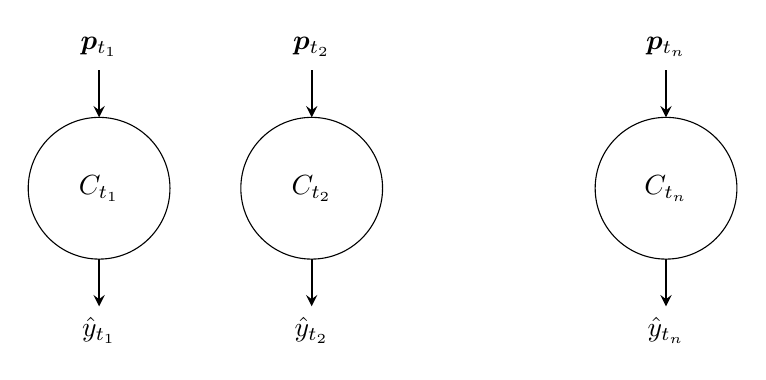
\begin{tikzpicture}[scale=0.3]
		\draw (1,5) circle (3cm);
		\node at (1,5) {$C_{t_1}$};
		\draw (10,5) circle (3cm);
		\node at (10,5) {$C_{t_2}$};
		\draw (25,5) circle (3cm);
		\node at (25,5) {$C_{t_n}$};
		\draw [arrow] (1,10)--(1,8);
		\draw [arrow] (10,10)--(10,8);
		\draw [arrow] (25,10)--(25,8);
		\node at (1,11) {$\bm{p}_{t_1}$};
		\node at (10,11) {$\bm{p}_{t_2}$};
		\node at (25,11) {$\bm{p}_{t_n}$};
		\draw [arrow] (1,2)--(1,0);
		\draw [arrow] (10,2)--(10,0);
		\draw [arrow] (25,2)--(25,0);
		\node at (1,-1) {$\hat{y}_{t_1}$};
		\node at (10,-1) {$\hat{y}_{t_2}$};
		\node at (25,-1) {$\hat{y}_{t_n}$};
	\end{tikzpicture}
	\caption{$n$ independent classifiers}
	\label{fig:IndependentClassifiers}
\end{figure}

Note that each $C_{t_j}$ minimizes the loss function
\[
	\frac{1}{N} \sum_{i=1}^N \mathscr{L} ( \bm{p}^i_{t_j},y_i;\tilde{\beta}_j )  ,
\]
with $\tilde{\beta}_j = ( \tilde{\beta}_{j0}, \tilde{\beta}_{j1}, \tilde{\beta}_{j2}, \dots, \tilde{\beta}_{jl})^T$. If we stack $\tilde{\beta}_j$ in rows we get a resulting matrix  $\tilde{\beta}$ such that
\[
	\tilde{\beta} = \{ \tilde{\beta}_{jk} \} = \left[\tilde{\beta}_1, \tilde{\beta}_2, \ldots, \tilde{\beta}_n  \right]^T .
\]
The matrix $\tilde{\beta}$ can also be obtained by minimizing the loss function
\begin{equation}\label{eq:indepClass}
	\frac{1}{nN} \sum_{j=1}^n \sum_{i=1}^N  \mathscr{L} ( \bm{p}^i_{t_j},y_i;\tilde{\beta})  ,
\end{equation}
as $\{\bm{p}^i_{t_j}\}_{i=1}^N$ for a fixed age $t_j$ only affects $\tilde{\beta}_j$. Therefore the matrix $\tilde{\beta}$ can be computed row by row by minimizing $\sum_{i=1}^N \mathscr{L} \left( \bm{p}^i_{t_j},y_i;\tilde{\beta}_j \right)$ for each $j$. Thus, we can write
\begin{equation}\label{eq:4_2}
	\argmin_{\tilde{\beta}} \sum_{j=1}^n \sum_{i=1}^N \mathscr{L} ( \bm{p}^i_{t_j},y_i;\tilde{\beta} ) = \bigg[\argmin_{\tilde{\beta}_1} \sum_{i=1}^N \mathscr{L} ( \bm{p}^i_{t_1},y_i;\tilde{\beta}_1 ), \dots ,\argmin_{\tilde{\beta}_n} \sum_{i=1}^N \mathscr{L} ( \bm{p}^i_{t_n},y_i;\tilde{\beta}_n ) \bigg]^T \!\!.
\end{equation}
Thus, $n$ independent classifiers $\{C_{t_j}\}_{j=1}^n$ minimize the loss function given in equation \eqref{eq:indepClass}.

Having $n$ independent classifiers $\left\{C_{t_j}\right\}_{j=1}^n$ is sub-optimal because the partial observations at ages $t_j$ are not  independent from those aged $t_{j-1}$ and $t_{j+1}$. Thus  the classifier $C_{t_j}$ can benefit from the knowledge of $C_{t_{j+1}}$ and vice-versa. Furthermore, the partial observations of an event change little from $t_j$ to $t_{j+1}$. Taking these into account,  we modify the original loss function given in equation \eqref{eq:indepClass} by including an $L_2$ penalty term as follows:
\begin{equation}\label{eq:ExtParCl_1}
	\varphi(\tilde{\beta}, \lambda ) = \frac{1}{nN} \sum_{j=1}^n  \sum_{i=1}^N \mathscr{L} ( \bm{p}^i_{t_j},y_i;\tilde{\beta} ) + \lambda \sum_{j=1}^{n-1} \left\lVert \tilde{\beta}_{j+1} - \tilde{\beta}_{j} \right\rVert ^2
\end{equation}
for some $\lambda >0 $, where $\lVert \cdot \rVert$ denotes the $L_2$ norm. The constant $\lambda$ is a parameter that can be specified. Recall that $\tilde{\beta}_j = \left(\tilde{\beta}_{j0}, \tilde{\beta}_{j1}, \tilde{\beta}_{j2}, \dots, \tilde{\beta}_{jl} \right)$ relates to partial observations $\{ \bm{p}^i_{t_j}\}_{i=1}^N$ for a fixed $t_j$, i.e.\ $\tilde{\beta}_{j0}$ is the coefficient of the intercept at age $t_j$ and $\tilde{\beta}_{j1}$ is the coefficient of the first covariate at age $t_j$. Thus the penalty term
\[
	\left\lVert \tilde{\beta}_{j+1} - \tilde{\beta}_{j} \right\rVert ^2 = \sum_{k=0}^l (\tilde{\beta}_{j+1,k} - \tilde{\beta}_{j,k})^2  ,
\]
and each term $(\tilde{\beta}_{j+1,k} - \tilde{\beta}_{j,k})^2$ takes coefficients for the $k$th covariate at ages $t_j$ and $t_{j+1}$ and penalizes the difference, enforcing a certain smoothness in event-age. The connected classifier CC minimizes this loss function. As a result of the $L_2$ penalty term, the individual classifiers are connected to form a single  classifier. Thus CC finds $\tilde{\beta}_*$ such that,
\begin{equation}\label{eq:ExtParCl_2}
	\tilde{\beta}_* = 	\argmin_{\tilde{\beta}} \bigg( \frac{1}{nN} \sum_{i=1}^N \sum_{j=1}^n \mathscr{L} ( \bm{p}^i_{t_j},y_i;\tilde{\beta} ) + \lambda \sum_{j=1}^{n-1} \left\lVert \tilde{\beta}_{j+1} - \tilde{\beta}_{j} \right\rVert ^2 \bigg)  .
\end{equation}

When $\lambda = 0$, CC is equivalent to $n$ independent classifiers as the cost function is reduced to that of equation~\eqref{eq:indepClass}. When $\lambda \to \infty$ the coefficients $\tilde{\beta}_{j+1} \to \tilde{\beta}_j$ to minimize the cost function. We recall that $\tilde{\beta}_j$ is the vector of coefficients of $C_{t_j}$. This gives rise to the same classifier for all event ages. Thus, CC is a connected classifier that is in between a single classifier and $n$ independent classifiers. A schematic diagram of CC is shown in Figure~\ref{fig:ConnectedClassifiers}.

\begin{figure}[!htb]
	\centering
	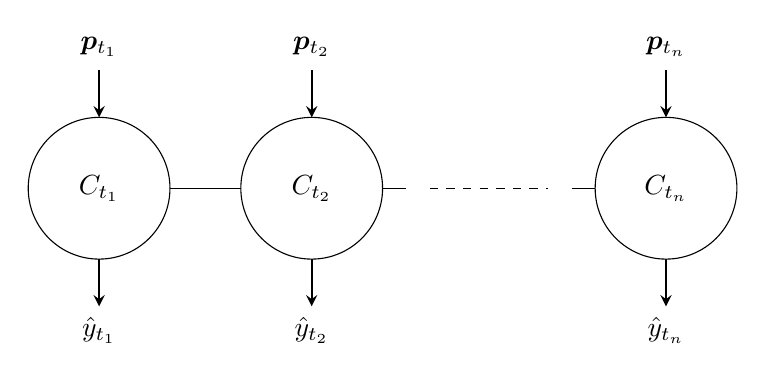
\begin{tikzpicture}[scale=0.3]
		\draw (1,5) circle (3cm);
		\node at (1,5) {$C_{t_1}$};
		\draw (10,5) circle (3cm);
		\node at (10,5) {$C_{t_2}$};
		\draw (25,5) circle (3cm);
		\node at (25,5) {$C_{t_n}$};
		\draw [arrow] (1,10)--(1,8);
		\draw [arrow] (10,10)--(10,8);
		\draw [arrow] (25,10)--(25,8);
		\node at (1,11) {$\bm{p}_{t_1}$};
		\node at (10,11) {$\bm{p}_{t_2}$};
		\node at (25,11) {$\bm{p}_{t_n}$};
		\draw [arrow] (1,2)--(1,0);
		\draw [arrow] (10,2)--(10,0);
		\draw [arrow] (25,2)--(25,0);
		\node at (1,-1) {$\hat{y}_{t_1}$};
		\node at (10,-1) {$\hat{y}_{t_2}$};
		\node at (25,-1) {$\hat{y}_{t_n}$};
		\draw (4,5) -- (7,5);
		\draw (13,5) -- (14,5);
		\draw (21,5) -- (22,5);
		\draw[dashed] (15,5)--(20,5);
	\end{tikzpicture}
	\caption{A connected classifier.}
	\label{fig:ConnectedClassifiers}
\end{figure}

As any loss function $\mathscr{L}$ can be used in equation \eqref{eq:ExtParCl_2}, CC is a general formulation. Our implementation of CC in \textit{eventstream} \citep{eventstream} uses logistic regression as the base classifier and the associated loss function. However, CC can be implemented with any loss function. For logistic regression \citep{friedman2001elements} the loss function $\mathscr{L}$ is given by
\begin{equation}\label{eq:LogReg}
	\mathscr{L} (\bm{p}^i_{t_j},y_i;\tilde{\beta}) = - y_i \big( [ 1 ~~ ( \bm{p}^i_{t_j})^T] \tilde{\beta}_{j} \big) + \log \Big( 1+ \exp\big\{[ 1 ~~ ( \bm{p}^i_{t_j})^T ] \tilde{\beta}_{j}\big\} \Big)  .
\end{equation}
Here the vector $[1 ~~ ( \bm{p}^i_{t_j})^T]$ denotes the concatenation of the vector $\bm{p}^i_{t_j}$ with the constant $1$ to account for the intercept.

\subsection{Comparison with unlinked classifiers}

We refer to CC with logistic regression as CC-Log in the following sections and compare its performance with two configurations of logistic regression classifiers. The first configuration comprises a single classifier, which is trained on all partial observations and their ages $\left(t_i, \mathbf{p}_{t_i} \right)$ as shown in Figure~\ref{fig:SingleClassifier}. We refer to this configuration as $1$-Log in the following sections. The second configuration comprises $n$ independent classifiers as shown in Figure~\ref{fig:IndependentClassifiers}.  We refer to this configuration of $n$ independent classifiers as $n$-Log. The $n$-Log classifier comprises of $\{C_{t_j} \}_{j=1}^n$, where each $C_{t_j}$ is trained on partial observations of age $t_j$, i.e.\ $\{\bm{p}^i_{t_j}\}_{i=1}^N$.

\begin{figure}[!hbt]
	\centering
	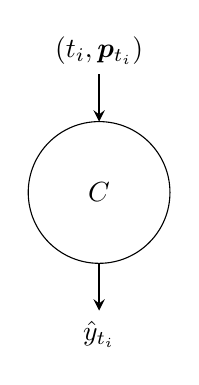
\begin{tikzpicture}[scale=0.3]
		\draw (1,5) circle (3cm);
		\node at (1,5) {$C$};
		\draw [arrow] (1,10)--(1,8);
		\node at (1,11) {$\left( t_i, \bm{p}_{t_i} \right)$};
		\draw [arrow] (1,2)--(1,0);
		\node at (1,-1) {$\hat{y}_{t_i}$};
	\end{tikzpicture}
	\caption{A Single classifier}
  \label{fig:SingleClassifier}
\end{figure}

The difference between $1$-Log and $n$-Log is the number of independent classifiers. The only difference between $n$-Log and CC-Log is the connections between the independent classifiers, brought about by the $L_2$ penalty term  $ \sum_{j=1}^{n-1}\left\lVert \tilde{\beta}_{j+1} - \tilde{\beta}_{j} \right\rVert ^2$. We compare CC-Log with $1$-Log and $n$-Log because we want to understand whether linking independent classifiers benefits early classification.

% \ifxyz Next we explore non-Gaussian state space models for partial observations. \fi

%  \ifxyz
% % =======================================================================
% % =======================================================================
% \subsection{DCC: Dynamic Connected Classifier}\label{sec:CascadedDLM}
% % =======================================================================

% We use non-Gaussian state space models as described in \citep{durbin1998time} and \citep{mccormick2012dynamic} to model partial observations, and the implementation in  R package \textit{dma} \citep{dma}. We start with the linear Gaussian state space models which are given by the following equations :
% \begin{align}
% 	y_t          & = Z_t \alpha_t + \varepsilon_t \, , \label{eq:DLM_1} \\
% 	\alpha_{t+1} & = T_t \alpha_t + R_t \eta_t \, , \label{eq:DLM_2}
% \end{align}
% where $\varepsilon_t \in \mathcal{N} \left(0, H_t\right)$ and $\eta_t \in \mathcal{N} \left(0, Q_t\right)$. %and $\alpha_1 \in \left(0, Q_t\right)$.
% Here $y_t$ is an $N$-dimensional vector of observations and $\alpha_t$ is a $(l+1)$-dimensional state vector. The matrices $Z_t$, $T_t$, $R_t$, $H_t$ and $Q_t$ are known at the beginning. Equation \eqref{eq:DLM_1} is called the ``observation equation'' and equation \eqref{eq:DLM_2}  the ``state equation''. When using state space models for dynamic regression, $\alpha_t$ denotes the coefficients which update dynamically.

% If $y_t$ is a binary response such that
% $$ y_t \sim \text{Bernoulli}(p_t) \, , $$
% equation \eqref{eq:DLM_1} changes as

% \begin{equation}\label{eq:GDLM_2}
% 	\text{logit}(p_t) =   Z_t \alpha_t \, ,              \\
% \end{equation}
% with logit function $f(t)=\log(t/(1-t))$, while keeping equation \eqref{eq:DLM_2} unchanged.

% \subsubsection{Modelling partial observations with DCC}

% We are interested in a growing prediction $\{\theta^j_{t_1}, \theta^j_{t_2}, \dots, \theta^j_{t_n} \}$ for partial observations $\{\bm{p}^j_{t_1},\bm{p}^j_{t_2}, \bm{p}^j_{t_3}, \ldots \bm{p}^j_{t_n}\}$ belonging to the same complete observation. Again, we note that for partial observations $\{\bm{p}^j_{t_1},\bm{p}^j_{t_2}, \bm{p}^j_{t_3}, \ldots \bm{p}^j_{t_n}\}$, the time stamps $(t_1, t_2, \ldots, t_n)$ denote the ages of the partial observations, not the time of occurrence.

% As state space models generally deal with time, for each age $t_k$ we use a separate state space model. However, for some cases it may benefit if there is communication between the models regarding the same observation. To add communication between the models, we bundle the partial observation $\bm{p}^j_{t_k}$ with the prediction output $\theta^j_{t_{k-1}}$ of the lower age model and use it as input for the age $t_k$ model.

% To explain this further, let us define $\bm{P}_{t_k} = \left[ \bm{p}^1_{t_k}\, \bm{p}^2_{t_k}\, \cdots \, \bm{p}^N_{t_k} \right]^T$ - an $l \times N$ matrix containing all partial observations of age $t_k$, $\bm{1} = \left[ 1, 1, \dots, 1\right]^T$ and $\theta_{t_k} = \left[\theta^1_{t_k}, \theta^2_{t_k}, \dots, \theta^N_{t_k} \right]^T$ - the logit predictions of the partial observations in $\bm{P}_{t_k}$, where $\bm{p}^j_{t_k}$ is an $l$-vector and $N$ denotes the number of complete observations.

% Then the equation corresponding to equation \eqref{eq:GDLM_2} for the initial model for age $t_1$ can be written as

% \begin{align}
% 	\theta_{t_1} & = Z_{t_1} \alpha_{t_1} \, . \label{eq:OurMod2}                     \\
% 	\text{with} \qquad
%       Z_{t_1} & = [ \bm{1} \, \, \bm{P}_{t_1} ] \, , \label{eq:OurMod1}
% \end{align}
% Using the output $\theta_{t_1}$, we write the model for age $t_2$ as
% \begin{align}
% 	Z_{t_2}      & = [ \bm{1} \, \, \bm{P}_{t_2} \, \, \theta_{t_1}] \, ,\label{eq:OurMod3} \\
% 	\theta_{t_2} & = Z_{t_2} \alpha_{t_2} \, . \label{eq:OurMod4}
% \end{align}
% Building in this way we obtain
% \begin{align}
% 	Z_{t_k}      & = [ \bm{1} \, \, \bm{P}_{t_k} \, \, \theta_{k_{t-1}}] \, , \label{eq:OurMod5} \\
% 	\theta_{t_k} & = Z_{t_k} \alpha_{t_k} \, . \label{eq:OurMod6}
% \end{align}
% The equations \eqref{eq:OurMod5}, \eqref{eq:OurMod6} and \eqref{eq:DLM_2} describe the model for the partial observations at age $t_k$. Let us denote the model which describes the partial observations of age $t_k$ by $\Lambda_k$ and the predicted output using the inverse link function by $\hat{\bm{y}}_{t_k}$. Our Dynamic Connected Classifier (DCC) incorporates a series of sub-models $\{ \Lambda_k\}_{k=1}^n$ in its implementation. Figure~\ref{fig:PODLM} shows DCC with internal communications between sub-models $\Lambda_{k}$ and $\Lambda_{k+1}$.

% \begin{figure}[!hb]
% 	\centering
% 	\includegraphics[clip=true,scale=0.8]{./Graphics/Lots_of_circles_3.pdf}
% 	\caption{Structure of DCC with communication.}
% 	\label{fig:PODLM}
% \end{figure}

% However, communication between models $\Lambda_{k}$ and $\Lambda_{k+1}$ may not improve the overall accuracy for every partial observations problem. For example, for a class imbalanced problem, a small number of incorrect predictions in $\theta_{t_{k}}$ can have an adverse effect on the model $\Lambda_{k+1}$. Therefore, for some instances such as class imbalanced datasets, it is desirable for DCC  to have no communications between the sub-models $\Lambda_k$ and $\Lambda_{k+1}$ as shown in Figure~\ref{fig:PODLM2}.

% \begin{figure}[!hb]
% 	\centering
% 	\includegraphics[clip=true,scale=0.8]{./Graphics/Lots_of_circles_4.pdf}
% 	\caption{Structure of DCC without communication.}
% 	\label{fig:PODLM2}
% \end{figure}

% \fi

% =======================================================================
\section{Event classification results}\label{sec:Experiments}
% =======================================================================

We explore three groups of datasets in this Section: synthetic, fibre optic  and \ch{NO2} data. For each application, we use CC-Log, $1$-Log and $n$-Log to classify events extracted by CPDBEE algorithm. For all three applications we  use $\lambda= 0.05$ for consistency. The R code applicable to this section is available in the supplementary material. The data is either included in the R package \textit{eventstream} or can be generated using its functionality.

\subsection{Synthetic data}\label{subsec:ResultsSynthetic}

\begin{figure}
	\centering
	\subfloat[][]{
		\includegraphics[width=0.49\textwidth, trim=0 70 0 85, clip=true]{./Graphics/Events_100040.pdf}
	}
	\subfloat[][]{
		\includegraphics[width=0.49\textwidth, trim=0 70 0 85, clip=true]{./Graphics/Events_100044.pdf}
	}
	\caption{Two windows of data and extracted events.}
  \label{fig:TwoWindows}
\end{figure}

We generate a data stream of dimension $3500 \times 250$, of which $80\%$ $(2800 \times 250)$ is used for training and the remaining $20\%$ for testing. We use a moving window  of dimension $200 \times 250$ which moves by a step of $8 \times 250$. For each window we extract events  using CPDBEE algorithm as shown in Figure~\ref{fig:TwoWindows}. As class A events can have a maximum age of $30$, we use $4$ event ages for the classification tasks at $t = 8, 16, 24$ and $32$ time units, i.e.\ event features are calculated at these ages. For synthetic data classification, we do not use features which were motivated from the fibre optic example, i.e.\ we do not use features 11 and 12 from the list in Section~\ref{sec:Featurelist}, for computational efficiency. Furthermore, the centroid is not used in any classification task.

To obtain unbiased estimates, we repeat this experiment $5$ times using different seeds for data generation. We measure the classification accuracy, which is defined as $1 - $ misclassification error. Table~\ref{tab:Results_Synthetic} gives the mean and standard deviation of test set classification accuracy for the 3 classifiers, which shows that \ifxyz both \fi CC-Log \ifxyz and DCC \fi surpasses $1$-Log and $n$-Log classifiers. Also we see that all 3 classifiers improve their average accuracy levels with the age of the events with the exception of $n$-Log at $t_4$.

\begin{table}[!ht]
	\centering
	\begin{tabular}{llccccccccc}
		\toprule
		Accuracy Measure        & Classifier & \multicolumn{4}{c}{Accuracy} &       & \multicolumn{4}{c}{Standard deviation}                                                \\
		\cmidrule{3-6} \cmidrule{8-11}
		                        &            & $t_1$                        & $t_2$ & $t_3$                                  & $t_4$ &      & $t_1$ & $t_2$ & $t_3$ & $t_4$ \\
		\midrule
		Classification Accuracy & CC-Log     & 0.79                         & 0.88  & 0.91                                   & 0.91  &      & 0.13  & 0.11  & 0.10  & 0.08  \\
		\ifxyz   DCC            & 0.72       & 0.89                         & 0.90  & 0.92                                   &       & 0.20 & 0.05  & 0.06  & 0.03          \\ \fi
		                        & $1$-Log    & 0.71                         & 0.85  & 0.88                                   & 0.87  &      & 0.20  & 0.13  & 0.13  & 0.11  \\
		                        & $n$-Log    & 0.76                         & 0.84  & 0.89                                   & 0.51  &      & 0.12  & 0.11  & 0.07  & 0.28  \\

		\bottomrule
	\end{tabular}
	\caption{Mean and standard deviation of classification accuracy over $5$ repetitions.}
  \label{tab:Results_Synthetic}
\end{table}

\subsubsection{Significance results}
To determine if there is a  significant difference between the three classifiers, we conduct a Friedman test  on classification accuracy results. The Friedman test on classification accuracy results gave a $p$-value of $0.0156$,  showing that the classifiers are different at 5\% level of significance. To ascertain which methods perform better we conduct a Nemenyi test on classification accuracy results.

Figure~\ref{fig:NemenyiSynthetic} shows the  resulting Nemenyi plot of ranks with a 90\% level of confidence. Lower rank values indicate better performing methods. Blue coloured boxes indicate methods which do not differ significantly from each other. From Figure~\ref{fig:NemenyiSynthetic} we see that CC-Log is best suited for this data followed by $1$-Log and $n$-Log, with no significant difference between the two latter methods.

\begin{figure}[!ht]
	\centering
	\includegraphics[width=0.49\textwidth]{./Graphics/Nemenyi_Synthetic_Accuracy.pdf}
	\caption{Nemenyi plot for synthetic data using classification accuracy results.}
  \label{fig:NemenyiSynthetic}
\end{figure}

\subsection{Fibre optic cable data results}\label{sec:FibreOpticExperimentResults}

The fibre optic dataset is a $379 \times 587$ matrix as shown in Figure~\ref{fig:Real_World_Data_Stream}. We use a moving window model with a window size $40 \times 587$ and a step size $10 \times 587$ to extract events and compute features. For each window we extract  events using CPDBEE and use CC-Log, $1$-Log and $n$-Log to classify them. \ifxyz and DCC.\fi We use event ages $t = 10, 20, 30$ and $40$, because the maximum event-age is $40$ time units.

As the fibre optic dataset has 4 class A events, we use $4$-fold cross validation. The events extracted from the data stream is  divided into four folds with each fold containing one class A event resembling Figure~\ref{fig:FourFolds}.

This modified form of cross validation is commonly used for time dependent observations \citep{watersurrogates} as in a streaming data scenario. The classifiers CC-Log, \ifxyz DCC \fi $1$-Log and $n$-Log are trained on events comprising of 3 training folds, and tested on the remaining fold.

\begin{figure}
	\centering
	\includegraphics[width=0.49\textwidth]{./Graphics/4Fold_CV.pdf}
	\caption{Data chunks for 4-fold cross validation.}
  \label{fig:FourFolds}
\end{figure}

As this dataset has a smaller number of class A events compared to class B events, we report additional accuracy measures that are designed for imbalanced datasets. We compute the positive predictive value (PPV) and the negative predictive value (NPV) and area under the receiver operator characteristic curve (AUC).
We give the definitions of these metrics below:
\[
	\text{Positive predictive value (PPV)} = \frac{\text{Number of true positives}}{\text{Number of predicted positives}}  ,
\]
\[
	\text{Negative predictive value (NPV)} = \frac{\text{Number of true negatives}}{\text{Number of predicted negatives}}  .
\]
The number of predicted positives in PPV is the sum of true positives and false positives, and the number of predicted negatives in NPV is the sum of true negatives and the false negatives. Considering PPV and NPV together gives a two-sided accuracy measure. For example, a classifier that predicts all observations as negative except for one correct positive observation achieves a PPV of $100\%$ but a small NPV\@. The combination of PPV and NPV gives the overall accuracy of the model.

In contrast, AUC is a single measure that captures the effectiveness of a classifier. The receiver operator characteristic (ROC) curve is a plot of the true positive rate against the false positive rate for different classification thresholds. The area under the curve (AUC) provides a measure of discrimination between positive and negative classes. The AUC does not depend on the classification threshold as it is an aggregate measure. An AUC closer to 1 is reflective of a good model, while a random predictor will give an AUC closer to 0.5. The AUC can be interpreted as the probability that a positive observation is ranked higher than a negative observation.

\begin{table}[!htb]
	\centering
	\begin{tabular}{llccccccccc}
		\toprule
		Accuracy Measure & Classifier & \multicolumn{4}{c}{Mean} &       & \multicolumn{4}{c}{Standard deviation}                                            \\
		\cmidrule{3-6} \cmidrule{8-11}
		                 &            & $t_1$                    & $t_2$ & $t_3$                                  & $t_4$ &  & $t_1$ & $t_2$ & $t_3$ & $t_4$ \\
		\midrule
		PPV              & CC-Log     & 1.00                     & 1.00  & 1.00                                   & 0.95  &  & 0.0   & 0.0   & 0.00  & 0.1   \\
		\ifxyz           & DCC        & 0.74                     & 0.69  & 0.68                                   & 0.68  &  & 0.18  & 0.15  & 0.12  & 0.23  \\ \fi
		                 & $1$-Log    & 0.81                     & 0.73  & 0.73                                   & 0.73  &  & 0.21  & 0.32  & 0.32  & 0.32  \\
		                 & $n$-Log    & 0.90                     & 1.00  & 0.93                                   & 1.00  &  & 0.20  & 0.0   & 0.12  & 0.0   \\
		\midrule
		NPV              & CC-Log     & 0.92                     & 0.94  & 0.95                                   & 0.95  &  & 0.03  & 0.03  & 0.03  & 0.03  \\
		\ifxyz           & DCC        & 0.98                     & 1.00  & 0.99                                   & 1.00  &  & 0.02  & 0.00  & 1.00  & 0.00  \\ \fi
		                 & $1$-Log    & 0.95                     & 0.96  & 0.95                                   & 0.93  &  & 0.01  & 0.02  & 0.05  & 0.06  \\
		                 & $n$-Log    & 0.97                     & 0.92  & 0.96                                   & 0.96  &  & 0.02  & 0.03  & 0.02  & 0.03  \\
		\midrule
		AUC              & CC-Log     & 0.96                     & 0.97  & 0.97                                   & 0.95  &  & 0.01  & 0.01  & 0.01  & 0.06  \\
		\ifxyz           & DCC        & 0.94                     & 0.97  & 0.94                                   & 0.97  &  & 0.07  & 0.00  & 0.05  & 0.01  \\ \fi
		                 & $1$-Log    & 0.88                     & 0.84  & 0.84                                   & 0.83  &  & 0.09  & 0.15  & 0.15  & 0.13  \\
		                 & $n$-Log    & 0.93                     & 0.96  & 0.94                                   & 0.98  &  & 0.09  & 0.01  & 0.05  & 0.01  \\
		\bottomrule
	\end{tabular}
	\caption{Mean and standard deviation of PPV, NPV and AUC $(\%)$ over $4$ folds.}
  \label{tab:AverageAccuracyReal}
\end{table}

Table~\ref{tab:AverageAccuracyReal} gives the average PPV, NPV and AUC values with their standard deviations over the $4$-folds for the fibre-optic data stream. For PPV and NPV, we use a probability threshold of $0.5$; i.e.\ if the output probability is greater than 0.5, it is deemed class A, and class B otherwise.

\ifxyz A high PPV signifies a low false positive rate and a high NPV, a low false negative rate. From Table~\ref{tab:AverageAccuracyReal}, we see that SCC has the highest average PPV and DCC has the highest average NPV for all event ages.  Of the two classifiers, SCC is more conservative in predicting class A events compared with the DCC\@. That is, if SCC predicts an event as belonging to class A, it is more likely that the actual event is of class A compared with DCC\@. This is supported by the high mean PPV values and the associated low standard deviations of SCC\@. On the other hand, DCC is much more likely to catch all class A events compared with SCC  as seen by the higher NPV values, i.e.\ there may be more false positives but a low number of false negatives indicate that class A events are unlikely to be labelled as class B. Whether it is better to be conservative and miss some class A events while being very accurate in terms of the predicted class A events, or to identify all class A events while giving some false positives, depends on the application. Often the cost of  false positives and false negatives are not the same; for example consider a medical test for cancer. Thus, we see that our proposed two models have different strengths. In addition, both these models outperform the logistic regression classifier as seen by the AUC values. \fi

\subsubsection{Significance results}
Friedman tests on  AUC, PPV and NPV results  gave $p$-values of  $0.0048$, $0.0045$ and $ 0.7583$ respectively. This shows that while AUC and PPV results differ significantly across classifiers, NPV results are similar. As such, we conduct Nemenyi tests on AUC and PPV values. Figure~\ref{fig:FibreNemenyi} shows Nemenyi test ranks for PPV and AUC, with lower ranks denoting better performance.

From Figure~\ref{fig:FibreNemenyi1} we see that for PPV CC-Log outperforms $n$-Log and $n$-Log outperforms $1$-Log with a 95\% level of confidence. For AUC results, both CC-Log and $n$-Log significantly outperform $1$-Log. Even though CC-Log outperforms $n$-Log, the two classifiers are not significantly different from each other as depicted by the blue squares in Figure~\ref{fig:FibreNemenyi2}.

\begin{figure}[!htb]
	\centering
	\subfloat[][]{
		\includegraphics[width=0.49\textwidth]{./Graphics/Nemenyi_PPV_Fibre.pdf}
    \label{fig:FibreNemenyi1} % width=0.49\textwidth, height = 0.48\textheight
	}%
	\subfloat[][]{
		\includegraphics[width=0.49\textwidth]{./Graphics/Nemenyi_ROC_Fibre.pdf}
    \label{fig:FibreNemenyi2}
	}
	\caption{Nemenyi plots for fibre optic cable data using PPV and AUC results.}
  \label{fig:FibreNemenyi}
\end{figure}

As NPV results across the classifiers are not significantly different, we turn our attention to PPV and AUC results in Table~\ref{tab:AverageAccuracyReal}. We see that CC-Log performs better at earlier event ages compared to $n$-Log. Noting that the only difference between $n$-Log and CC-Log is the connections between the independent classifiers, this demonstrates the importance of the connections for early event classification. That is, the knowledge of ``older'' events aids classification of ``younger'' events.

\subsection{Nitrogen dioxide monitoring}\label{sec:NO2Exp}

We consider  monthly \ch{NO2}  data from March to June for a 10 year period from 2010 to 2019. These are three dimensional datasets with two spatial and one time dimension. First we extract events using CPDBEE for each year separately. Then we perform 10-fold cross validation by training CC-Log, $1$-Log and $n$-Log classifiers on event data of $9$ years and testing it on the remaining year's data.

The extracted events are three dimensional clusters of high \ch{NO2} levels spanning space and time. Events are extracted from a  data stream of $4 \times 180 \times 360$ array, where each $180 \times 360$ matrix corresponds to the \ch{NO2} levels of a given month. We use CPDBEE parameters  $\alpha = 0.97$, $\epsilon=2$ and $\text{minPts} = 20$.
Figure~\ref{fig:ClustersNO2March2018} shows two dimensional cross sections of the three dimensional  \ch{NO2} clusters in March and June 2018.

\begin{figure}[!hb]
	\centering
	\subfloat[][]{
		\includegraphics[width=0.49\textwidth]{./Graphics/Clusters_NO2_March_2018_With_Bndry.pdf}
		\label{fig:ClustersNO2March20181}
	}%
	\subfloat[][]{
		\includegraphics[width=0.49\textwidth]{./Graphics/Clusters_NO2_June_2018_With_Bndry.pdf}
		\label{fig:ClustersNO2March20182}
	}
	\caption{Events extracted from \ch{NO2} data from March to June 2018. Figures~\ref{fig:ClustersNO2March20181} and~\ref{fig:ClustersNO2March20182} show  two dimensional cross sections of the three dimensional \ch{NO2} clusters in March and June 2018. Colours do not reflect \ch{NO2} levels. Each event is depicted by a single colour.}
	\label{fig:ClustersNO2March2018}
\end{figure}

For each 3-dimensional event we compute features 1--10 and 14 from the list of features in Section~\ref{sec:Featurelist}. These features are chosen for ease of computation. \ch{NO2} clusters which have grown in average intensity during this time period  are assigned the class label $1$ and others  $0$. As some \ch{NO2} clusters only start in April we designate the value in April as the starting value for class label computation. Thus, the task is to detect if \ch{NO2} clusters grow in intensity as soon as possible.

Table~\ref{tab:AverageAccuracyNO2} gives the 10-fold cross validation test results on \ch{NO2} clusters. We see that CC-Log achieves better accuracy results compared to $n$-Log and $1$-Log, with the only exception that $1$-Log achieves slightly better results at $t_4$.

\begin{table}[!htb]
	\centering
	\begin{tabular}{llccccccccc}
		\toprule
		Accuracy Measure        & Classifier & \multicolumn{4}{c}{Mean} &       & \multicolumn{4}{c}{Standard deviation}                                            \\
		\cmidrule{3-6} \cmidrule{8-11}
		                        &            & $t_1$                    & $t_2$ & $t_3$                                  & $t_4$ &  & $t_1$ & $t_2$ & $t_3$ & $t_4$ \\
		\midrule
		Classification Accuracy & CC-Log     & 0.84                     & 0.81  & 0.90                                   & 0.88  &  & 0.08  & 0.12  & 0.07  & 0.07  \\
		                        & $1$-Log    & 0.80                     & 0.80  & 0.88                                   & 0.89  &  & 0.09  & 0.11  & 0.07  & 0.07  \\
		                        & $n$-Log    & 0.80                     & 0.80  & 0.87                                   & 0.83  &  & 0.09  & 0.12  & 0.06  & 0.11  \\
		\bottomrule
	\end{tabular}
	\caption{10-Fold Cross validation accuracy comparison on \ch{NO2} clusters.}
  \label{tab:AverageAccuracyNO2}
\end{table}

\subsubsection{Significance results}
Similar to the previous applications, we perform a Friedman test on the classification accuracy results. The Friedman test gave a $p$-value of $0.01752$, showing that there is a significant difference between the classifiers.

\begin{figure}[!htb]
	\centering
	\includegraphics[width=0.49\textwidth]{./Graphics/Nemenyi_Accuracy_NO2.pdf}
	\label{fig:Nemenyi_NO21} % width=0.49\textwidth, height = 0.48\textheight
	\caption{Nemenyi plot for \ch{NO2} data using classification accuracy results.}
	\label{fig:Nemenyi_NO2}
\end{figure}

Figure~\ref{fig:Nemenyi_NO2} shows the resulting Nemenyi plot, which shows that CC-Log outperforms $1$-Log and $n$-Log with a $5\%$ level of significance. The success of CC-Log demonstrates the benefit of linking classifiers that are trained on similar but slightly different data, on early event classification.

% =======================================================================
\section{Conclusions}\label{sec:Conclusions}
% =======================================================================

This paper has proposed a framework for event extraction and early event classification in contiguous spatio-temporal data streams. We  proposed an event detection and extraction algorithm as well as an early event classification algorithm. We  tested our event detection and classification framework using 3 applications, one synthetic and two real.

The event extraction algorithm CPDBEE uses change point detection and clustering techniques to detect and extract events. We compared CPDBEE with Kuldorff's Scan Statistic and achieved better results for all three applications in a much shorter time period.

The early event classification algorithm comprises of a set of base classifiers connected using an $L_2$ penalty term, inducing a certain level of smoothness in event age. We compared the connected classifier CC-Log, with two configurations of unlinked classifiers $1$-Log and $n$-Log and achieved better results for all three applications. Furthermore, for all three applications CC-Log achieved better results for early event ages. As the only difference between $n$-Log and CC-Log was the connections between the base classifiers, this reveals that classification of early events benefits from knowledge of more mature events. Future directions for this research include extending CPDBEE for non-contiguous spatio-temporal data as well as extending CC to use other base classifiers such as decision trees.

% =======================================================================
\section{Supplementary material}\label{sec:supmat}
% =======================================================================

\textbf{R-package eventstream:} This package contains CPDBEE algorithm for event extraction, the connected classifier CC-Log for early event classification, functions for synthetic data generation, the fibre-optic data stream and \ch{NO2} data. It is available from GitHub at \url{https://github.com/sevvandi/eventstream}.

\textbf{Scripts:} The file \url{Supp_Mat_CPDBEE} contains the code used in Section~\ref{sec:EventExtract}. There are three files containing the R code used in Section~\ref{sec:Experiments}. The files \url{Supp_Mat_1.R}, \url{Supp_Mat_2.R} and \url{Supp_Mat_3.R} contain the code applicable for synthetic data,  fibre optic data and \ch{NO2} data respectively.

\textbf{Other R-packages:} We have used the following R-packages either in this paper or within the package \textit{eventstream}:
  \textit{changepoint} \citep{killick2014changepoint},
  \textit{abind} \citep{abind},
  \textit{AtmRay} \citep{atmray},
  \textit{pROC} \citep{proc},
  \textit{ggplot2} \citep{ggplot2},
  \textit{raster} \citep{raster},
  \textit{maps} \citep{maps},
  \textit{tensorA} \citep{tensorA},
  \textit{glmnet} \citep{glmnet},
  \textit{dbscan} \citep{dbscan} and
  \textit{MASS} \citep{MASS}.

% =======================================================================
\section*{Acknowledgements}
% =======================================================================

Funding was provided by the Australian Research Council through the Linkage Project LP160101885.
%\newgeometry{top=0.5cm,bottom=0.5cm}
\newpage
\footnotesize\parskip=0cm
\bibliographystyle{agsm} %Choose a bibliograhpic style    IEEEtran
\bibliography{Master}

\newpage
% =======================================================================
\appendix
\section{Appendix}\label{sec:App1}
% =======================================================================

\subsection{Event extraction results for fibre optic cable data}

\begin{figure}[!htb]
	\centering
	\subfloat[][]{
		\includegraphics[width=0.42\textwidth]{./Graphics/Event_Comparison_1_40.pdf}
		\label{fig:events_1}
	}%
	\subfloat[][]{
		\includegraphics[width=0.42\textwidth]{./Graphics/Event_Comparison_41_80.pdf}
		\label{fig:events_2}
	}\\
	\subfloat[][]{
		\includegraphics[width=0.42\textwidth]{./Graphics/Event_Comparison_81_120.pdf}
		\label{fig:events_3}
	}%
	\subfloat[][]{
		\includegraphics[width=0.42\textwidth]{./Graphics/Event_Comparison_121_160.pdf}
		\label{fig:events_4}
	}
	\caption{Event extraction comparison for fibre optic data windows 1--6.}
  \label{fig:events_set1}
\end{figure}

% \restoregeometry
% \newgeometry{top=0.5cm,bottom=0.5cm}
\begin{figure}[!p]
	\centering
	\subfloat[][]{
		\includegraphics[width=0.42\textwidth]{./Graphics/Event_Comparison_161_200.pdf}
		\label{fig:events_5}
	}%
	\subfloat[][]{
		\includegraphics[width=0.42\textwidth]{./Graphics/Event_Comparison_201_240.pdf}
		\label{fig:events_6}
	} \\
	\subfloat[][]{
		\includegraphics[width=0.42\textwidth]{./Graphics/Event_Comparison_241_280.pdf}
		\label{fig:events_7}
	}%
	\subfloat[][]{
		\includegraphics[width=0.42\textwidth]{./Graphics/Event_Comparison_281_320.pdf}
		\label{fig:events_8}
	}\\
	\subfloat[][]{
		\includegraphics[width=0.42\textwidth]{./Graphics/Event_Comparison_321_360.pdf}
		\label{fig:events_9}
	}%
	\subfloat[][]{
		\includegraphics[width=0.42\textwidth]{./Graphics/Event_Comparison_361_379.pdf}
		\label{fig:events_10}
	}
	\caption{Event extraction comparison for fibre optic data windows 5--10.}
  \label{fig:events_set2}
\end{figure}

\newpage
\subsection{Event extraction results for synthetic data}

\begin{figure}[!htb]
	\centering
	\subfloat[][]{
		\includegraphics[width=0.49\textwidth]{./Graphics/Event_comparison_Synthetic_1_50.pdf}
		\label{fig:events_2_1}
	}%
	\subfloat[][]{
		\includegraphics[width=0.49\textwidth]{./Graphics/Event_comparison_Synthetic_51_100.pdf}
		\label{fig:events_2_2}
	}\\
	\subfloat[][]{
		\includegraphics[width=0.49\textwidth]{./Graphics/Event_comparison_Synthetic_101_150.pdf}
		\label{fig:events_2_3}
	}%
	\subfloat[][]{
		\includegraphics[width=0.49\textwidth]{./Graphics/Event_comparison_Synthetic_151_200.pdf}
		\label{fig:events_2_4}
	} \\
	\subfloat[][]{
		\includegraphics[width=0.49\textwidth]{./Graphics/Event_comparison_Synthetic_251_300.pdf}
		\label{fig:events_2_5}
	}%
	\subfloat[][]{
		\includegraphics[width=0.49\textwidth]{./Graphics/Event_comparison_Synthetic_301_350.pdf}
    \label{fig:events_2_6}
	}
	\caption{Event extraction comparison for synthetic data.}
	\label{fig:events_set_synthetic}
\end{figure}

\newpage

\subsection{Event extraction results for \ch{NO2} data}

\begin{figure}[!htb]
	\centering
	\subfloat[][]{
		\includegraphics[width=0.49\textwidth]{./Graphics/NO2_Event_Comparison_1_90_2.pdf}
		\label{fig:events_set_NO2_1}
	}%
	\subfloat[][]{
		\includegraphics[width=0.49\textwidth]{./Graphics/NO2_Event_Comparison_91_180_2.pdf}
		\label{fig:events_set_NO2_2}
	}\\
	\subfloat[][]{
		\includegraphics[width=0.49\textwidth]{./Graphics/NO2_Event_Comparison_181_270_2.pdf}
		\label{fig:events_set_NO2_3}
	}%
	\subfloat[][]{
		\includegraphics[width=0.49\textwidth]{./Graphics/NO2_Event_Comparison_271_360_2.pdf}
		\label{fig:events_set_NO2_4}
	}
	\caption{Event extraction comparison for \ch{NO2} data.}
  \label{fig:events_set_NO2}
\end{figure}

%1. A clustering approach for structural health monitoring on bridges \\
%2. Event Detection from Video Surveillance Data Based on Optical Flow Histogram and High-level Feature Extraction \\
% =======================================================================
\end{document}
% =======================================================================

%% Outline
%% 1. Introduction
%% 1.1		data streams - what is being done - literature
%% 1.2 		What they don't address
%% 1.3 What we do - a statistical approach for event classification
%% 2. Motivation & research problem
%% 2.1 		Real world example - early detection really important
%% 3 Notation - Our partial information model
%% 4. Partial observations classifiers
%%		- Explain the penalty and everything
%% 5. Cascaded Dynamic Linear Models for our work
%% 6. Datasets, Blob extraction, Features
%% 7 Results
%% 8. Future work and Conclusions
